\documentclass[11pt,letterpaper]{article}
\input{headings}
\newcommand \recipeName {Scalloped Potatoes}
\newcommand \fileName {ScallopedPotatoes}
\chead{\recipeName}

\begin{document}
\input{title}

Rather than a super-rich dish with heavy cream and cheese, I prefer a lighter version of scalloped potatoes. This recipe is inspired by one in Julia Child's {\it The Way to Cook} cookbook. I have tried to make this dish by simply replacing the heavy cream with whole milk. The problem is that the raw potato has an enzime that makes the milk curdle leading to an unappealing dish. The solution is to make a very light bechamel sauce first. The bonding of the milk with the butter and the flour prevents the curdling of the milk. 

\begin{description}

\item[Ingredients:]\ \\
	\begin{itemize}
	\item 2 1/2 pounds of Yukon gold or white potatoes
	\item 5 cups of milk
	\item 4 Tablespoons of butter
	\item 3 1/2 Tablespoons of flour (more to butter the baking dish)
	\item 2 teaspoons of salt
	\item 1/2 teaspoon of white pepper
	\item 1 clove of garlic
	\end{itemize}

\item[Optional Ingredients:]\ \\
	\begin{itemize}
	\item 1 1/2 Tablespoon of finely chopped chives
	\item 1 1/2 Tablespoon of finely chopped fresh sage
	\end{itemize}

\item[Procedure:]\ \\
	\begin{enumerate}
	\item {\bf Prepare the baking dish and pre-heat the oven.)}
		\begin{itemize}
		\item  Butter a baking dish.
		\item Preheat the oven to 375 F.
		\end{itemize}
	\item {\bf Make the Bechamel Sauce}
		\begin{itemize}
		\item Measure the milk in a large measuring glass dish.
		\item Heat the milk in a microwave.
		\item Meanwhile, melt the butter over moderate heat.
		\item Add the flour to the melted butter and stir with a whisk balloon cooking the flour but maintaining a blonde colour. 
		\item Remove from the fire and gently add the hot milk stirring vigorously in the beginning to prevent lumps from forming. 
		\item Once all the hot milk has been added, switch to a wood spoon. Cook, stirring, for a few minutes until the sauce thickens just slightly. It will be a thin sauce.
		\item Remove from the stove and let it cool just slightly while you prepare the seasoning for the sauce.
		\end{itemize}
	\item {\bf Season the sauce}
		\begin{itemize}
        		\item On a wood cutting board, using a chef's knive, crush the garlic. Then add the salt to the garlic and continue crushing until you obtain a paste.
		\item Add the white pepper to the paste and crush again.
		\item Add this paste to the warm sauce and stir well.
		\item If using, chop the herbs and add to the warm sauce. 	
		\end{itemize}
	\item {\bf Slice the potatoes and assemble the dish}
		\begin{itemize}
        		\item Using a food processor, slice the potatoes in 2.5 mm thick slices.
		\item Spoon a small amount of sauce on the bottom of the baking dish.
		\item Spread a layer of sliced potatoes and spread some sauce over that layer. You want to have enough sauce left over to completely cover the top of the dish with a thick layer of sauce.
		\item Spray a sheet of aluminum foil with cooking spray and cove the dish.
		\item Bake for at least one hour, or until a small sharp knife easily pierce the potatoes slices on the center of the dish.
		\end{itemize}
	\item{\bf Brown the top}
		\begin{itemize}
        		\item Increase the oven temperature to 400 F.
		\item Remove the aluminum foil from the top of the dish and return the dish to the oven.
		\item Bake for about 10 minutes until the top of the dish starts browning slightly.
		\item Remove from the oven, and let it cool for ten or fifteen minutes before serving.	
		\end{itemize} 	
     	\end{enumerate}         
\end{description}
\begin{table}
\begin{tabular}{cccc}
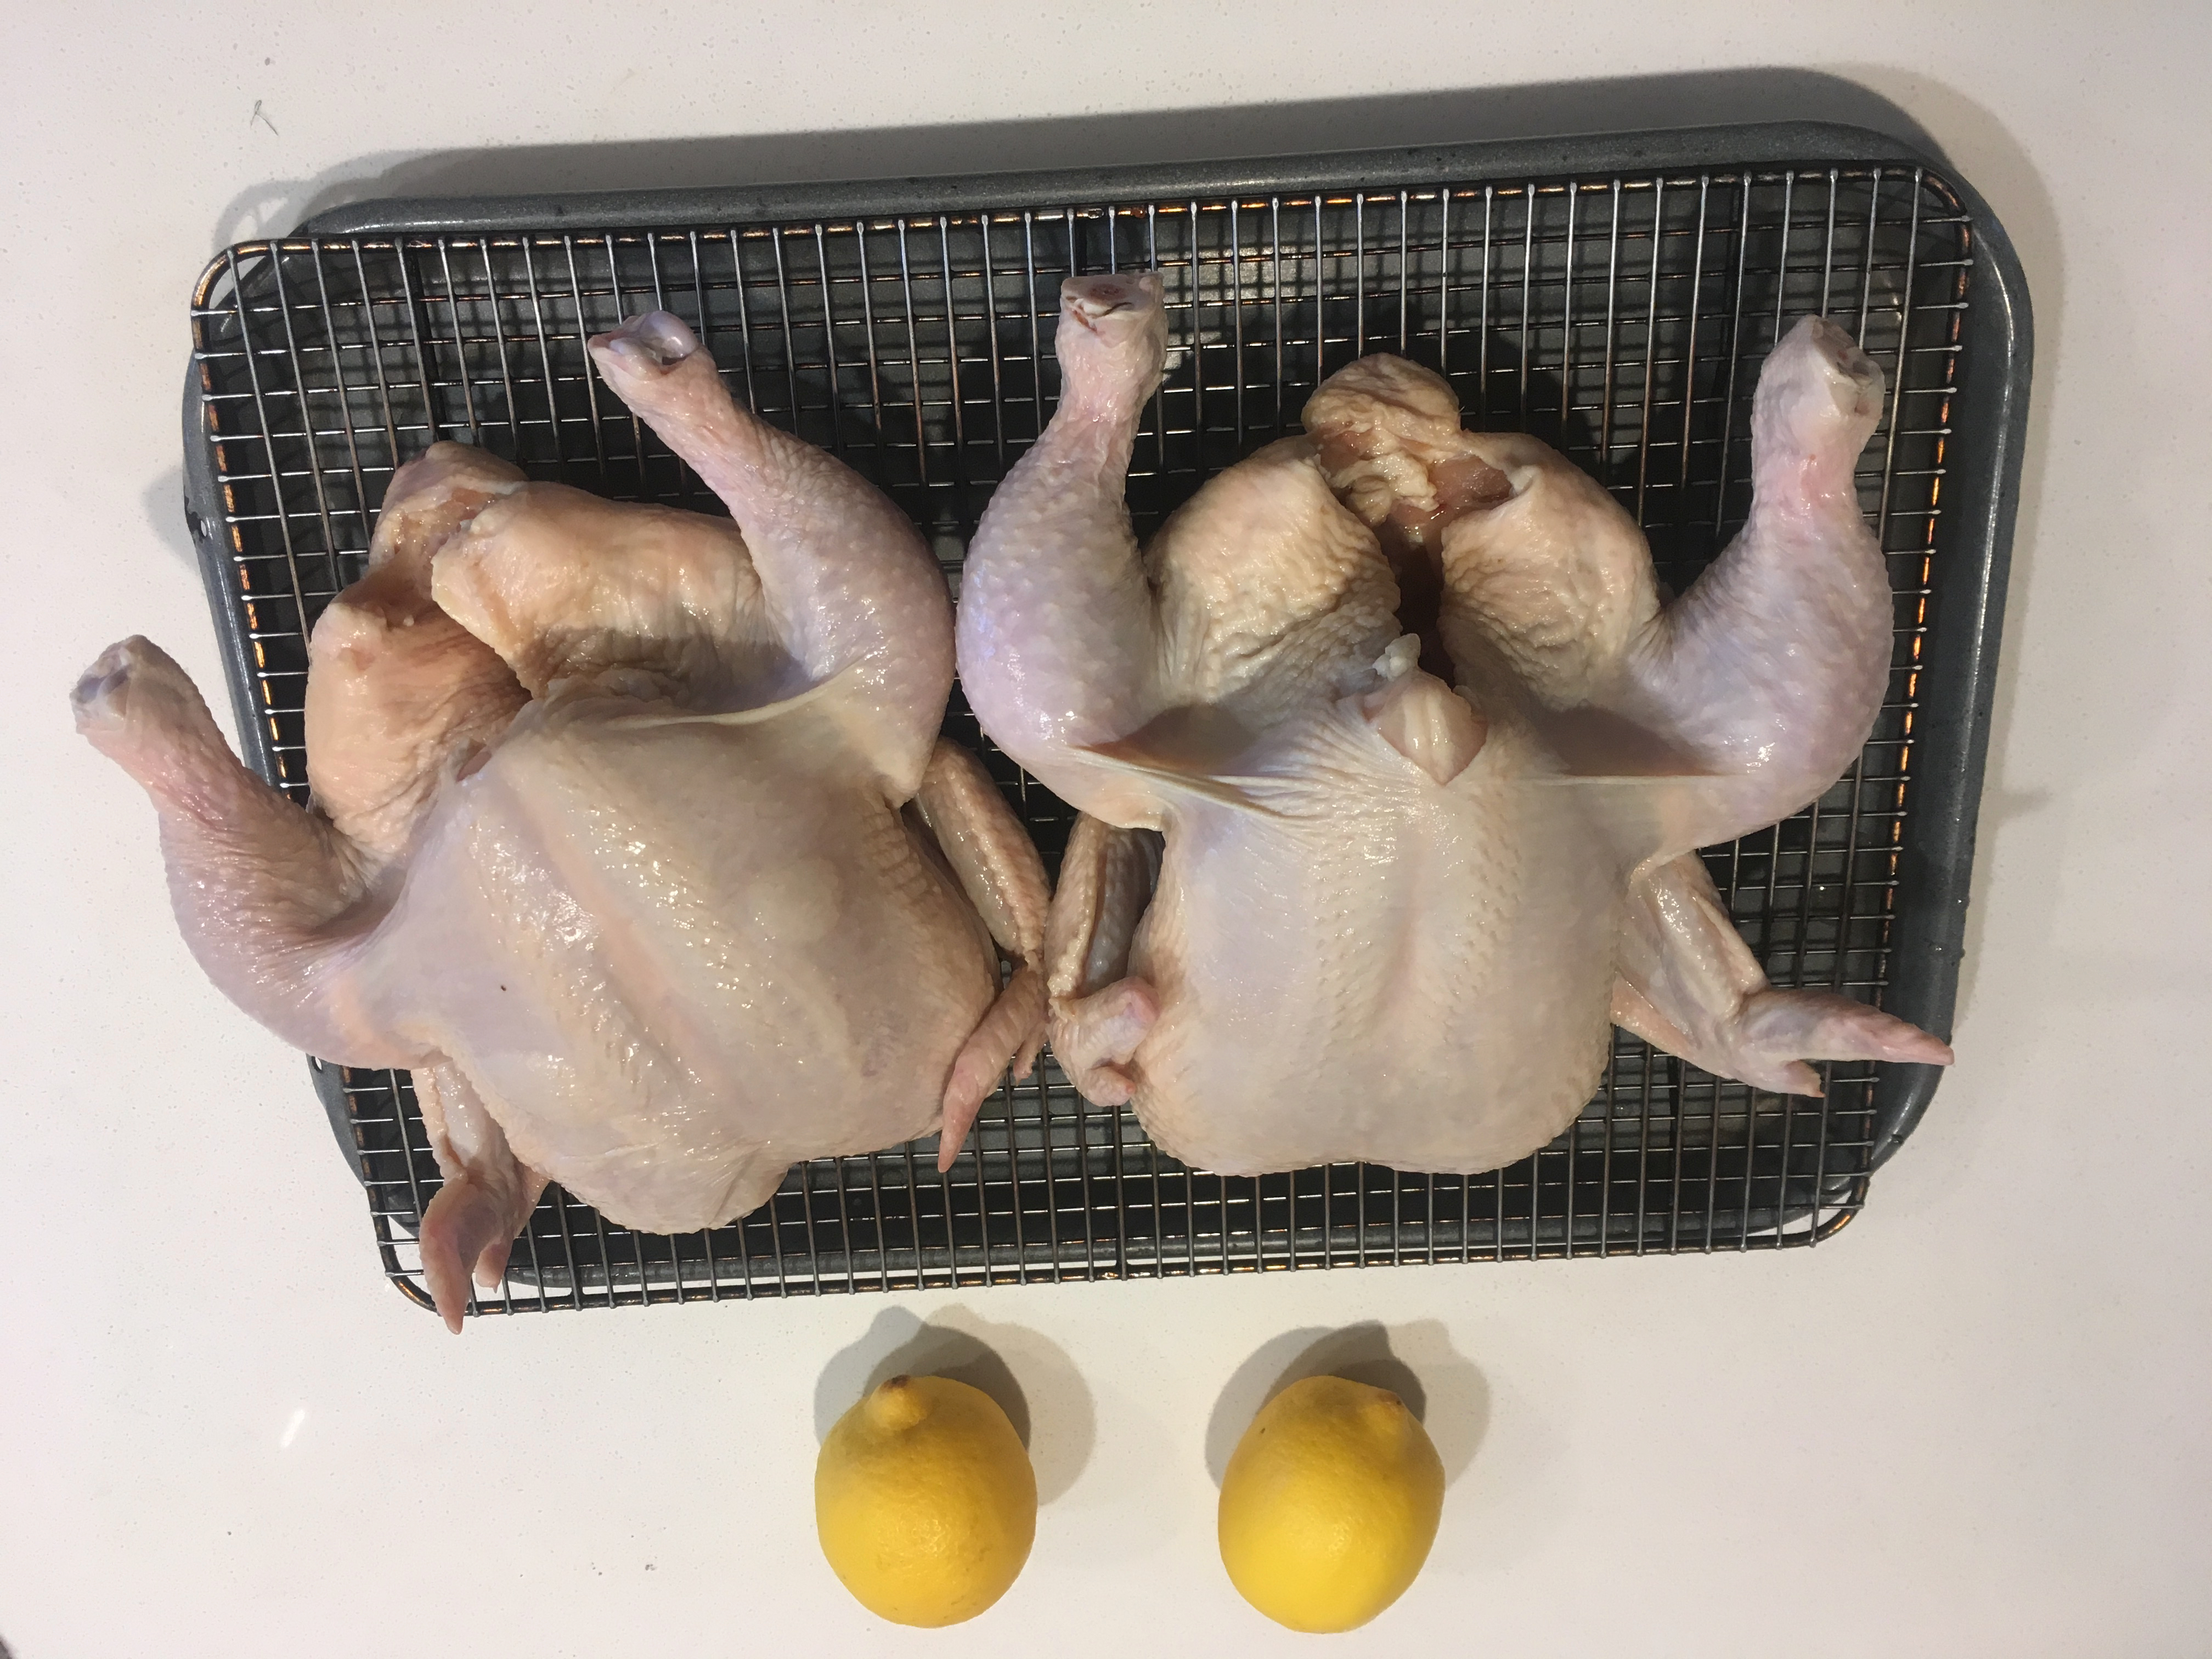
\includegraphics[width=0.25\textwidth]{\imageDir/\fileName/IMG_3197.jpg} &
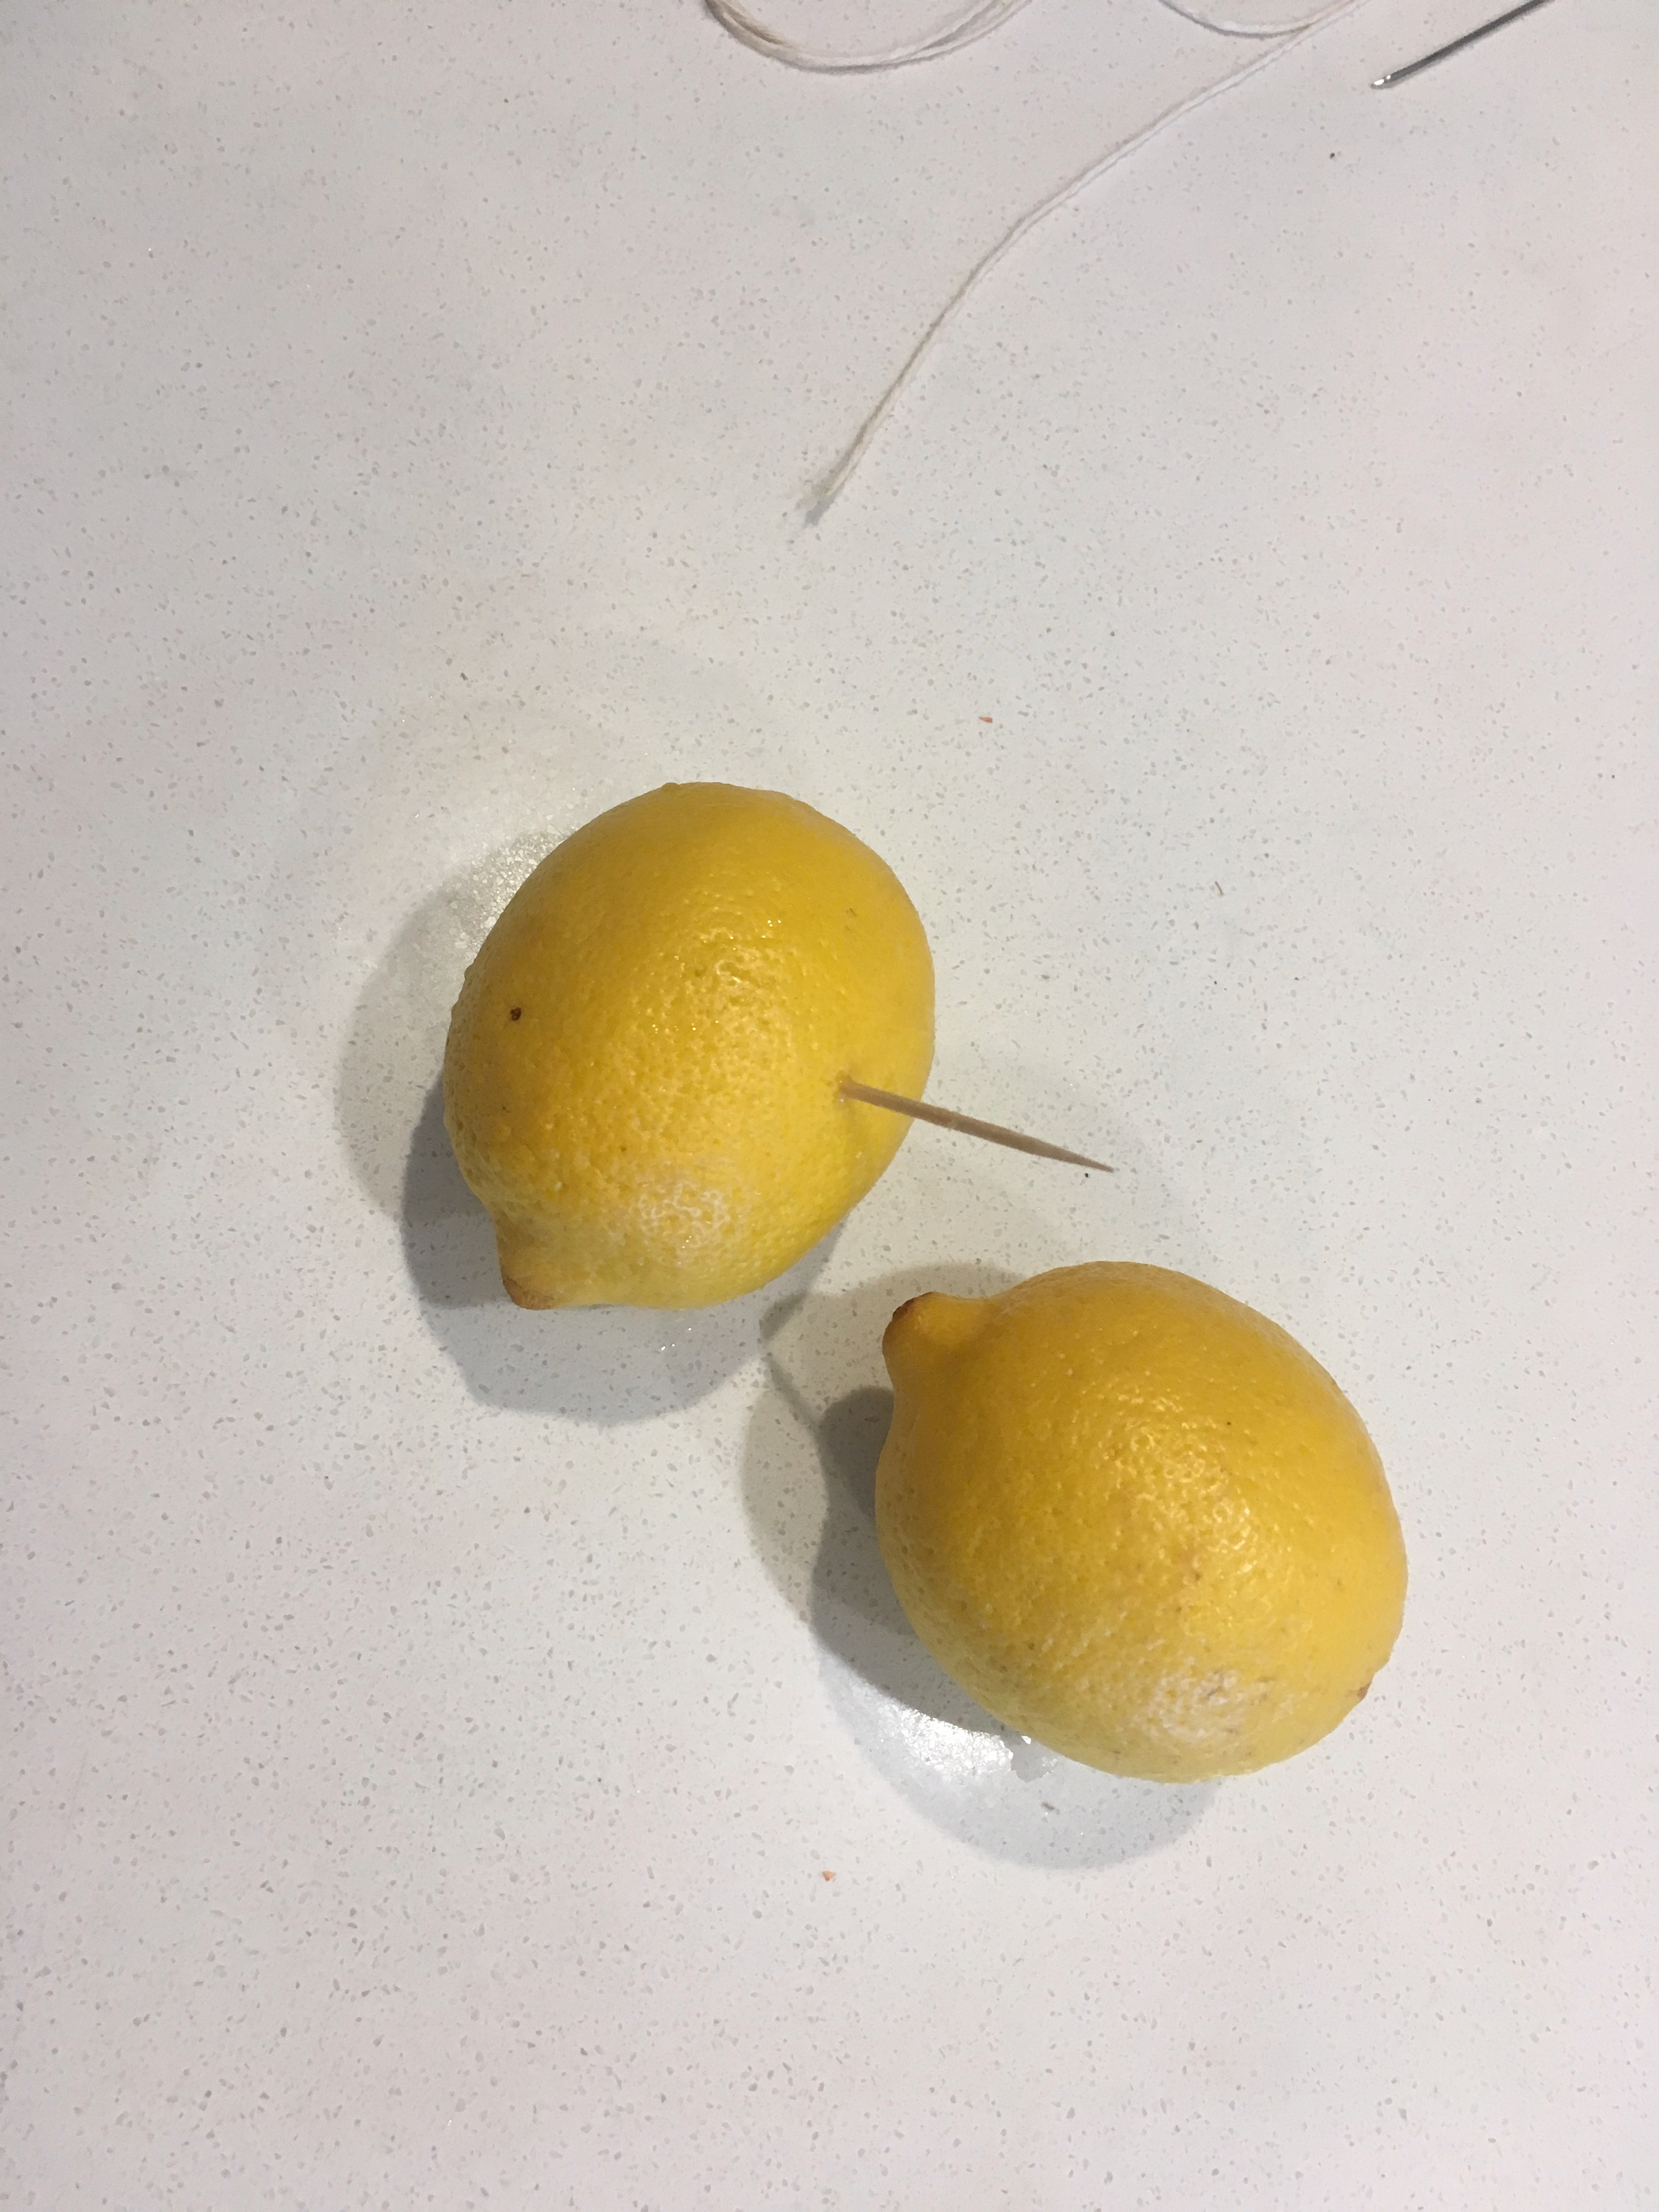
\includegraphics[width=0.25\textwidth]{\imageDir/\fileName/IMG_3212.jpg} &
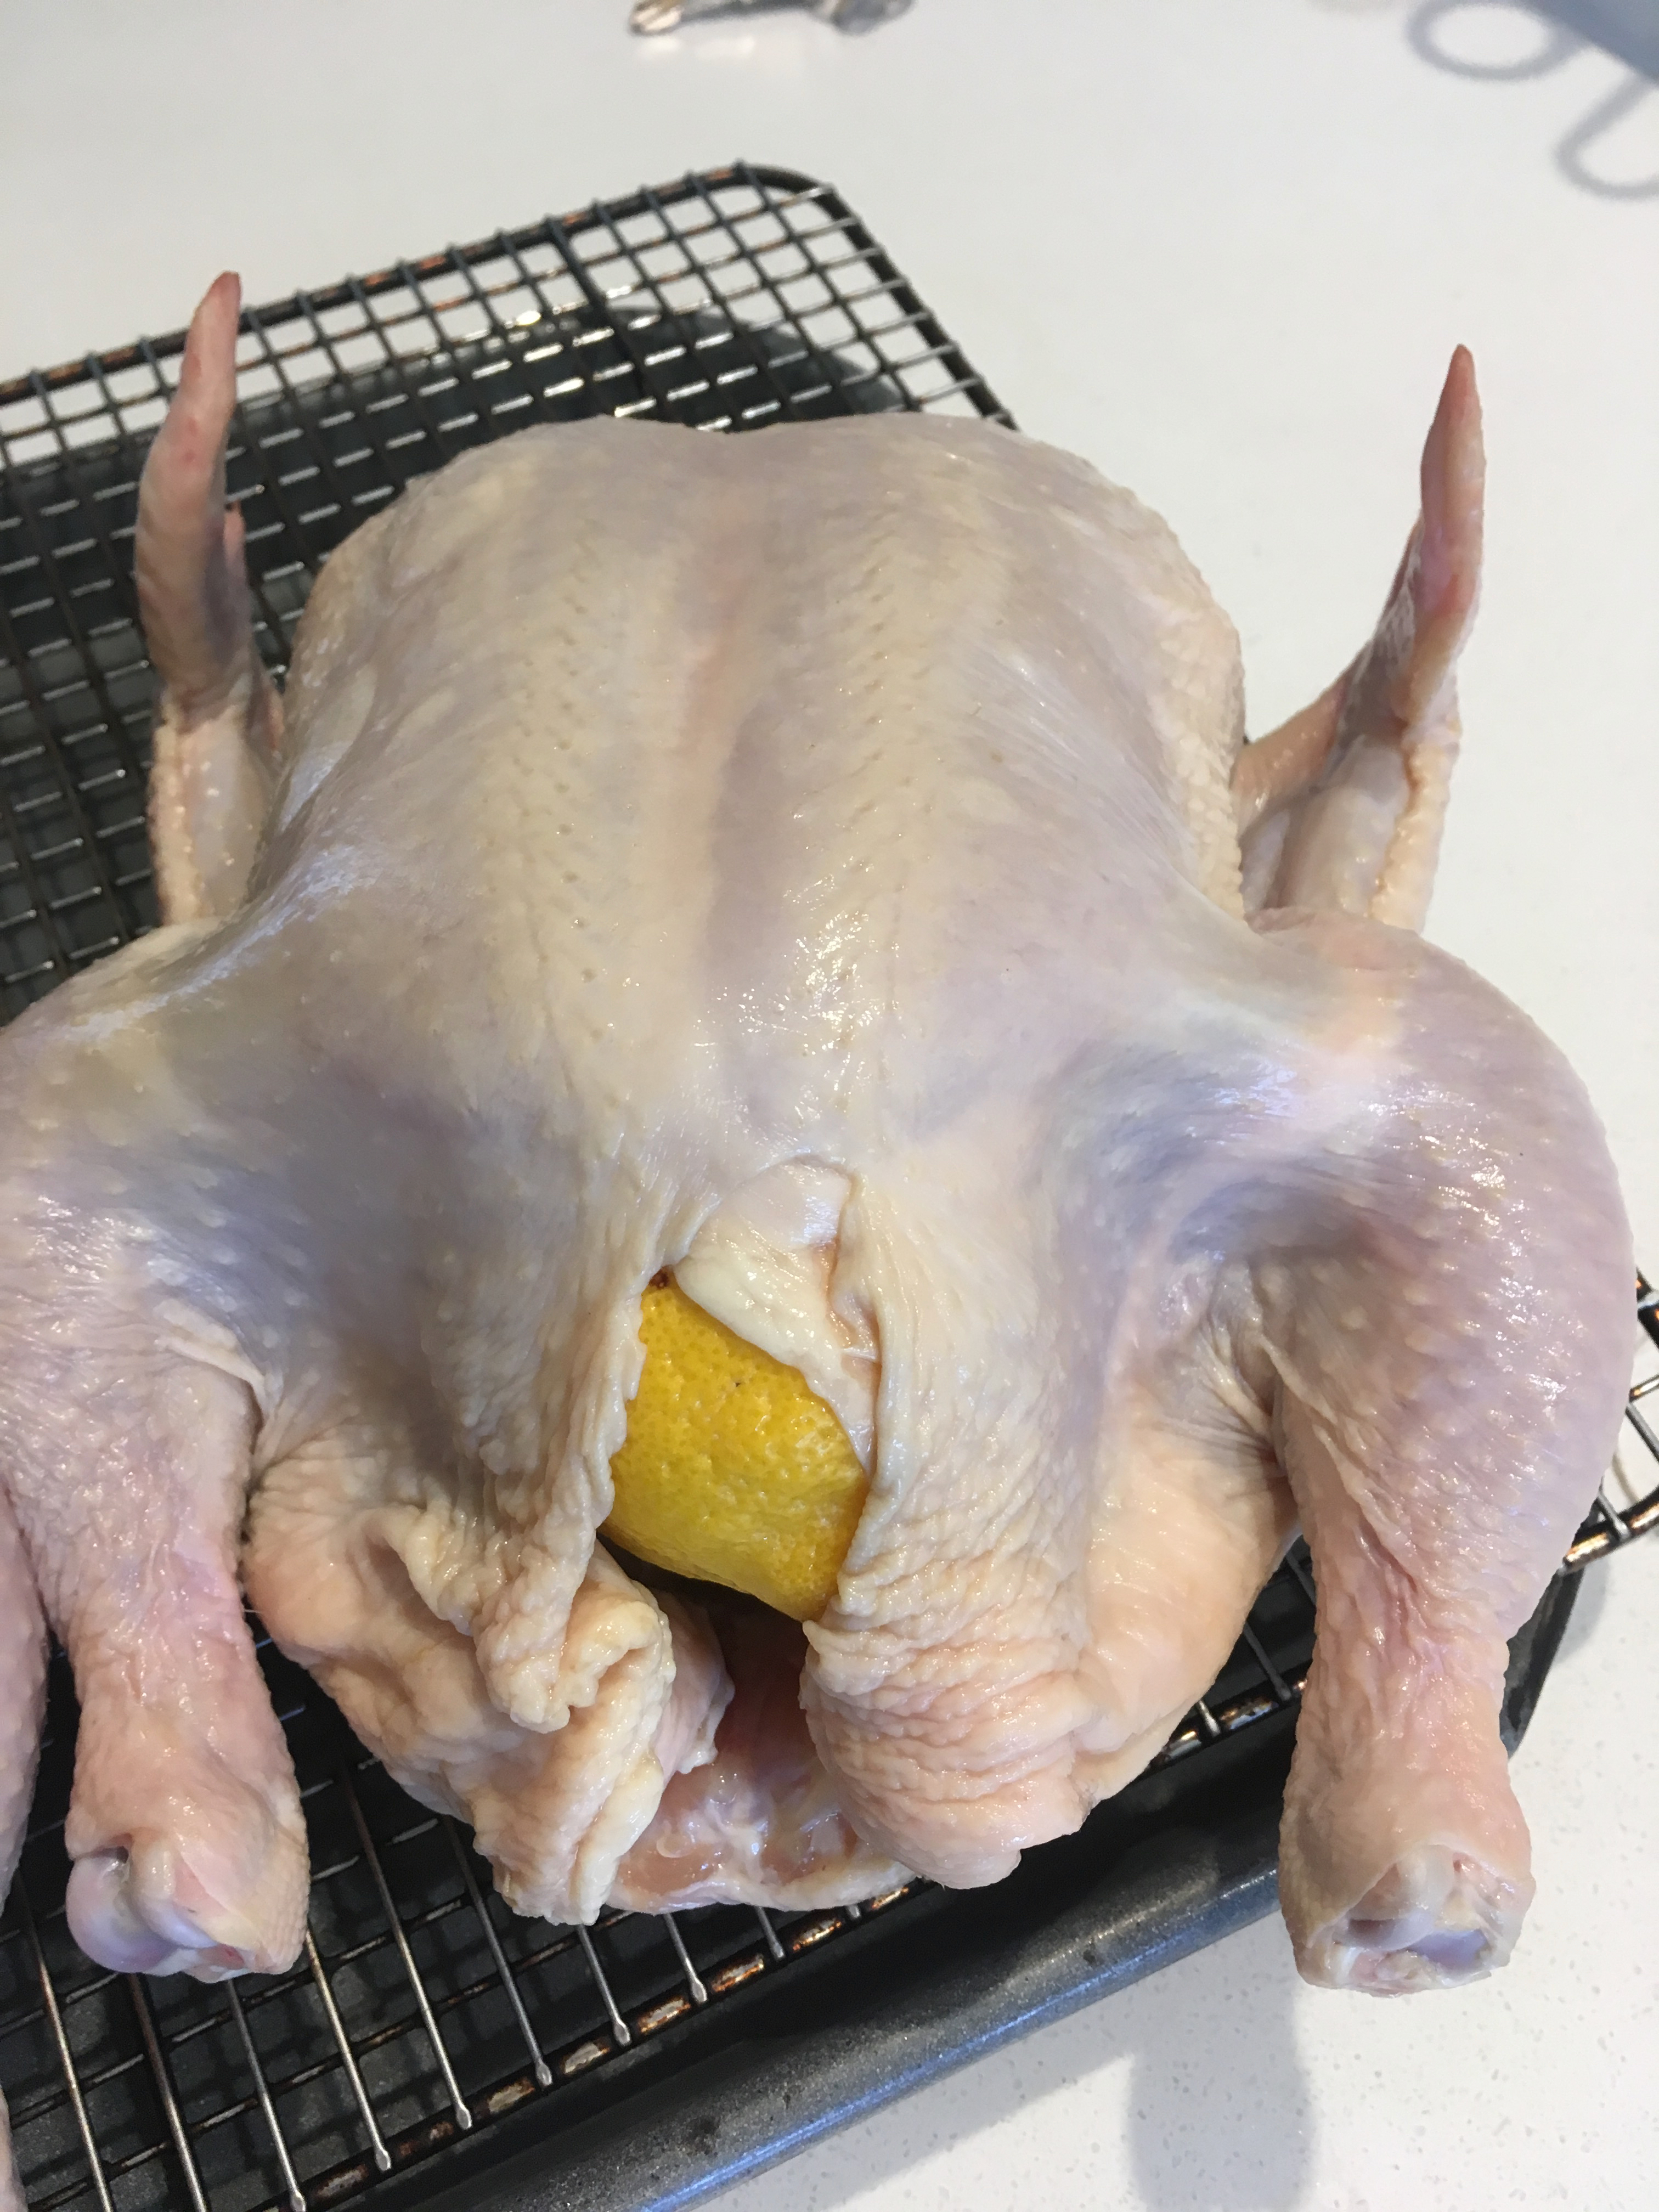
\includegraphics[width=0.25\textwidth]{\imageDir/\fileName/IMG_3213.jpg} \\
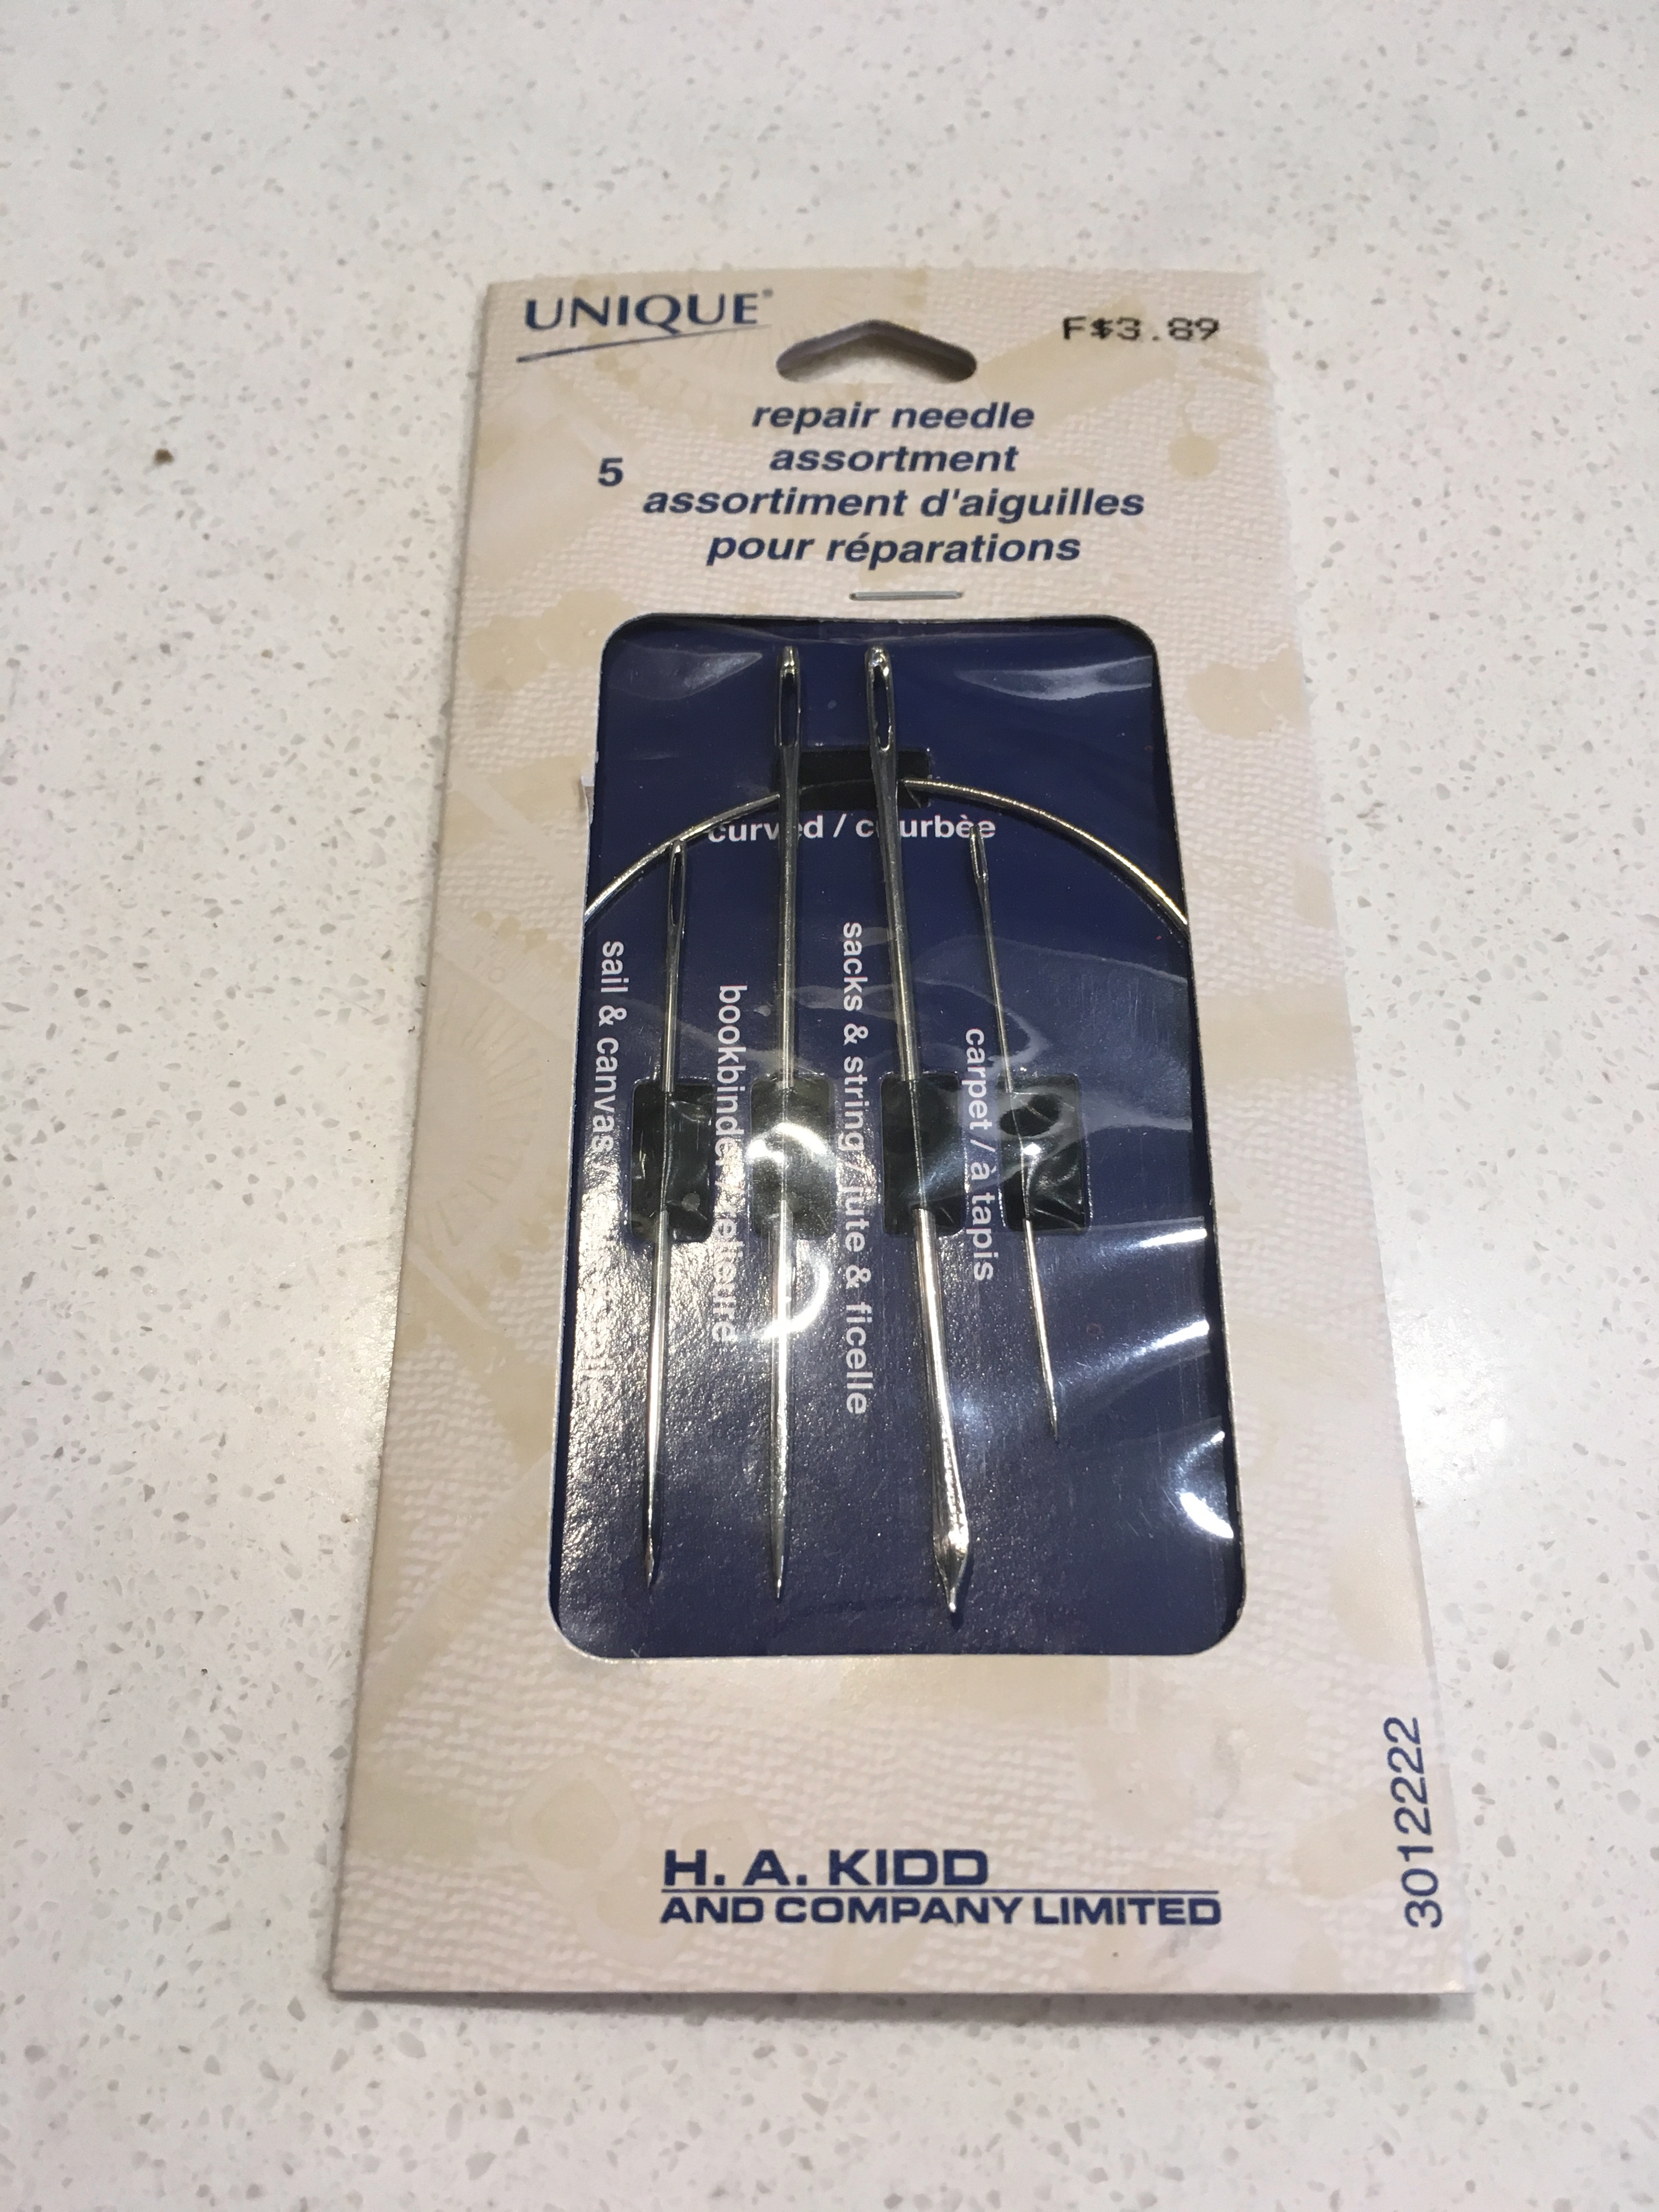
\includegraphics[width=0.25\textwidth]{\imageDir/\fileName/IMG_3206.jpg} &
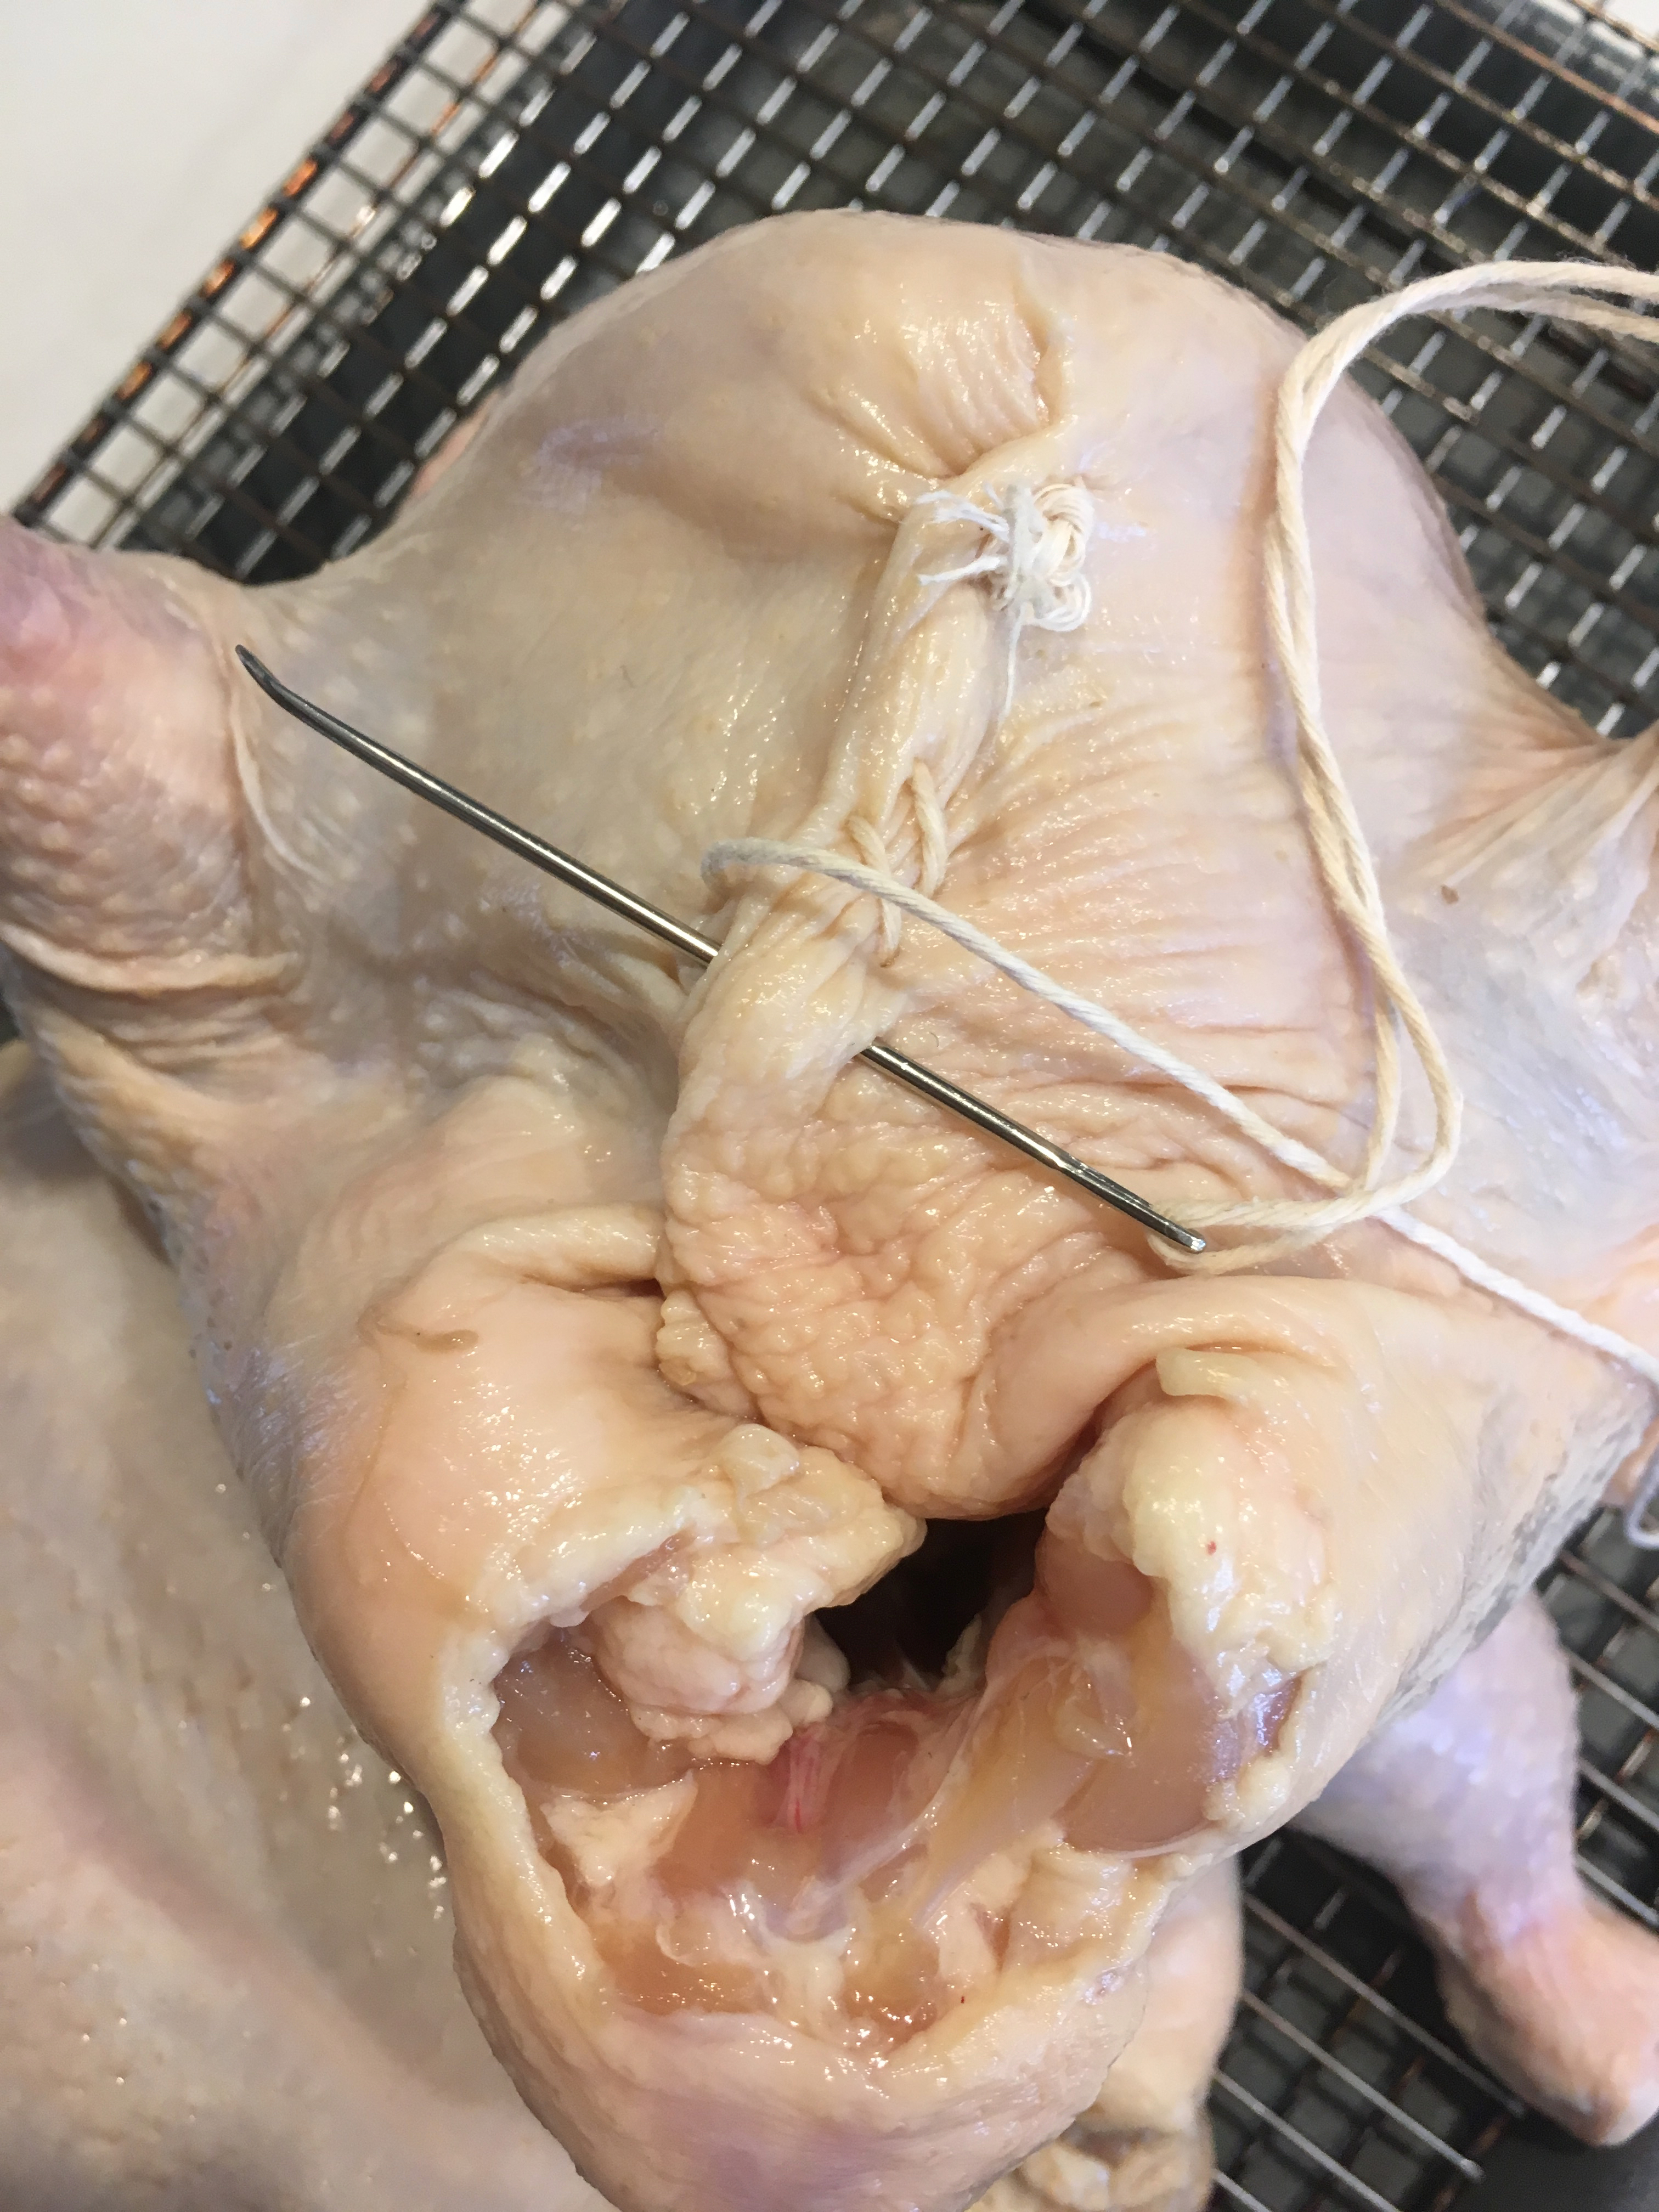
\includegraphics[width=0.25\textwidth]{\imageDir/\fileName/IMG_3214.jpg} &
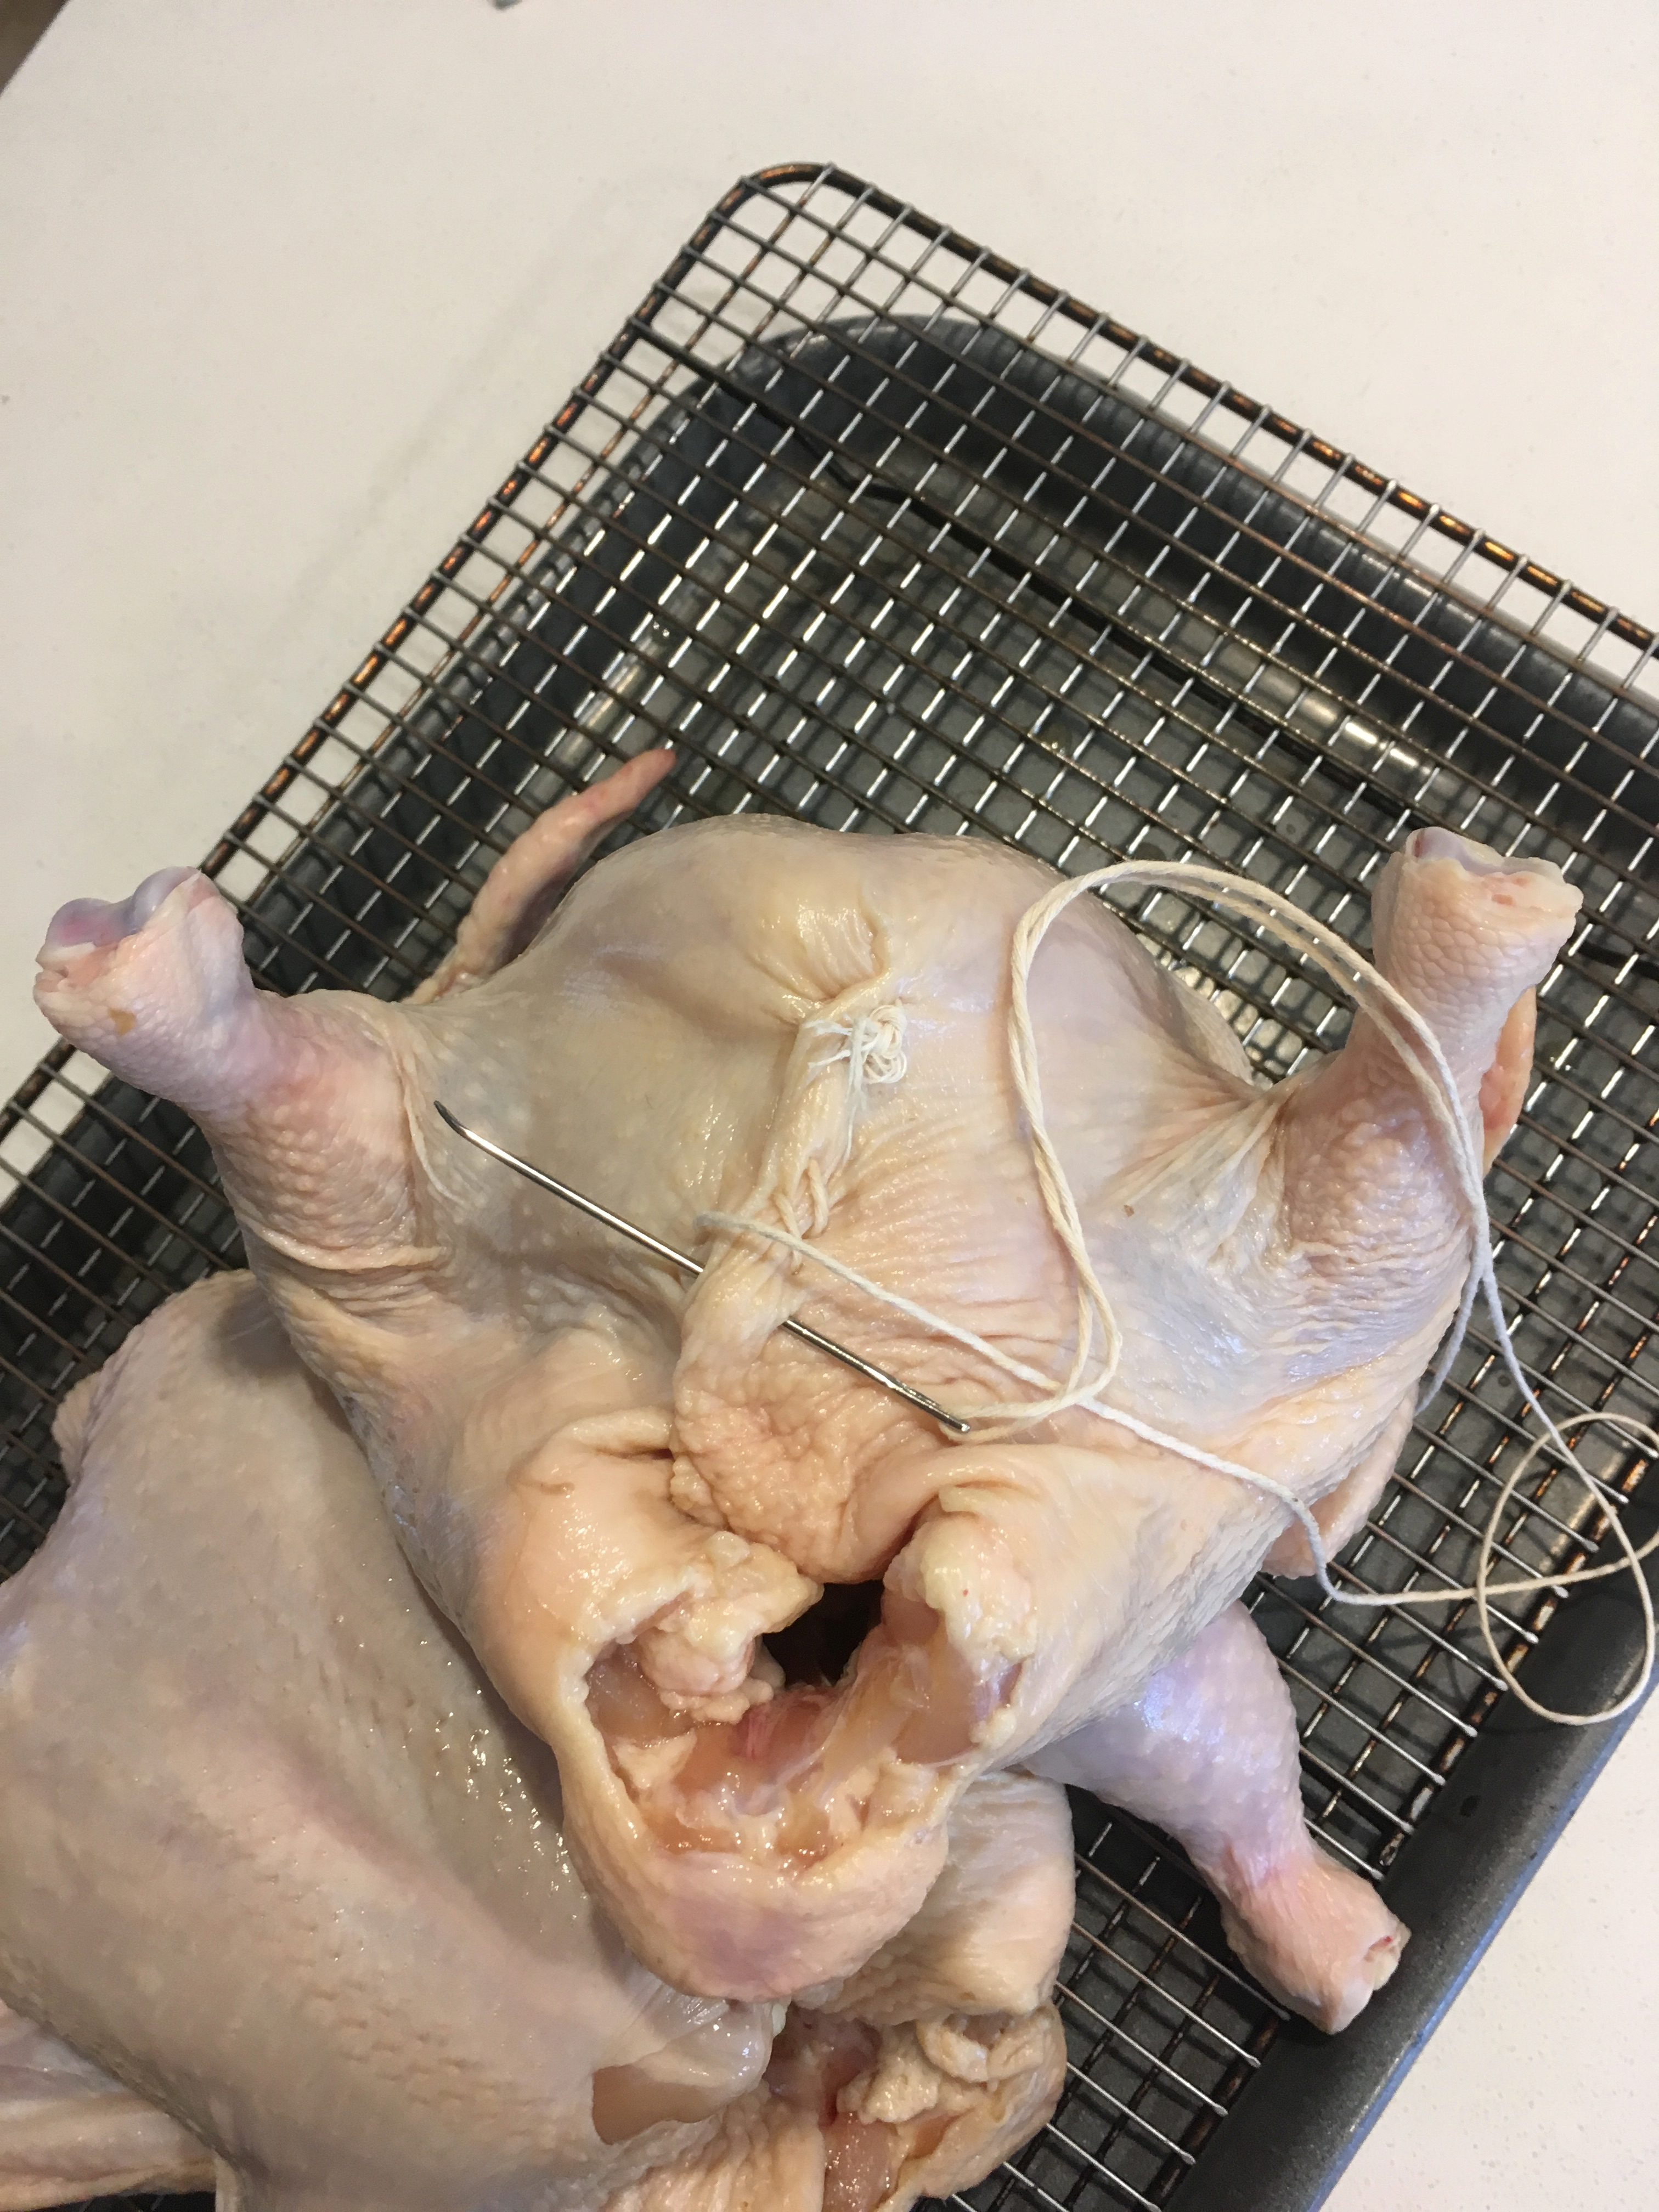
\includegraphics[width=0.25\textwidth]{\imageDir/\fileName/IMG_3216.jpg} \\
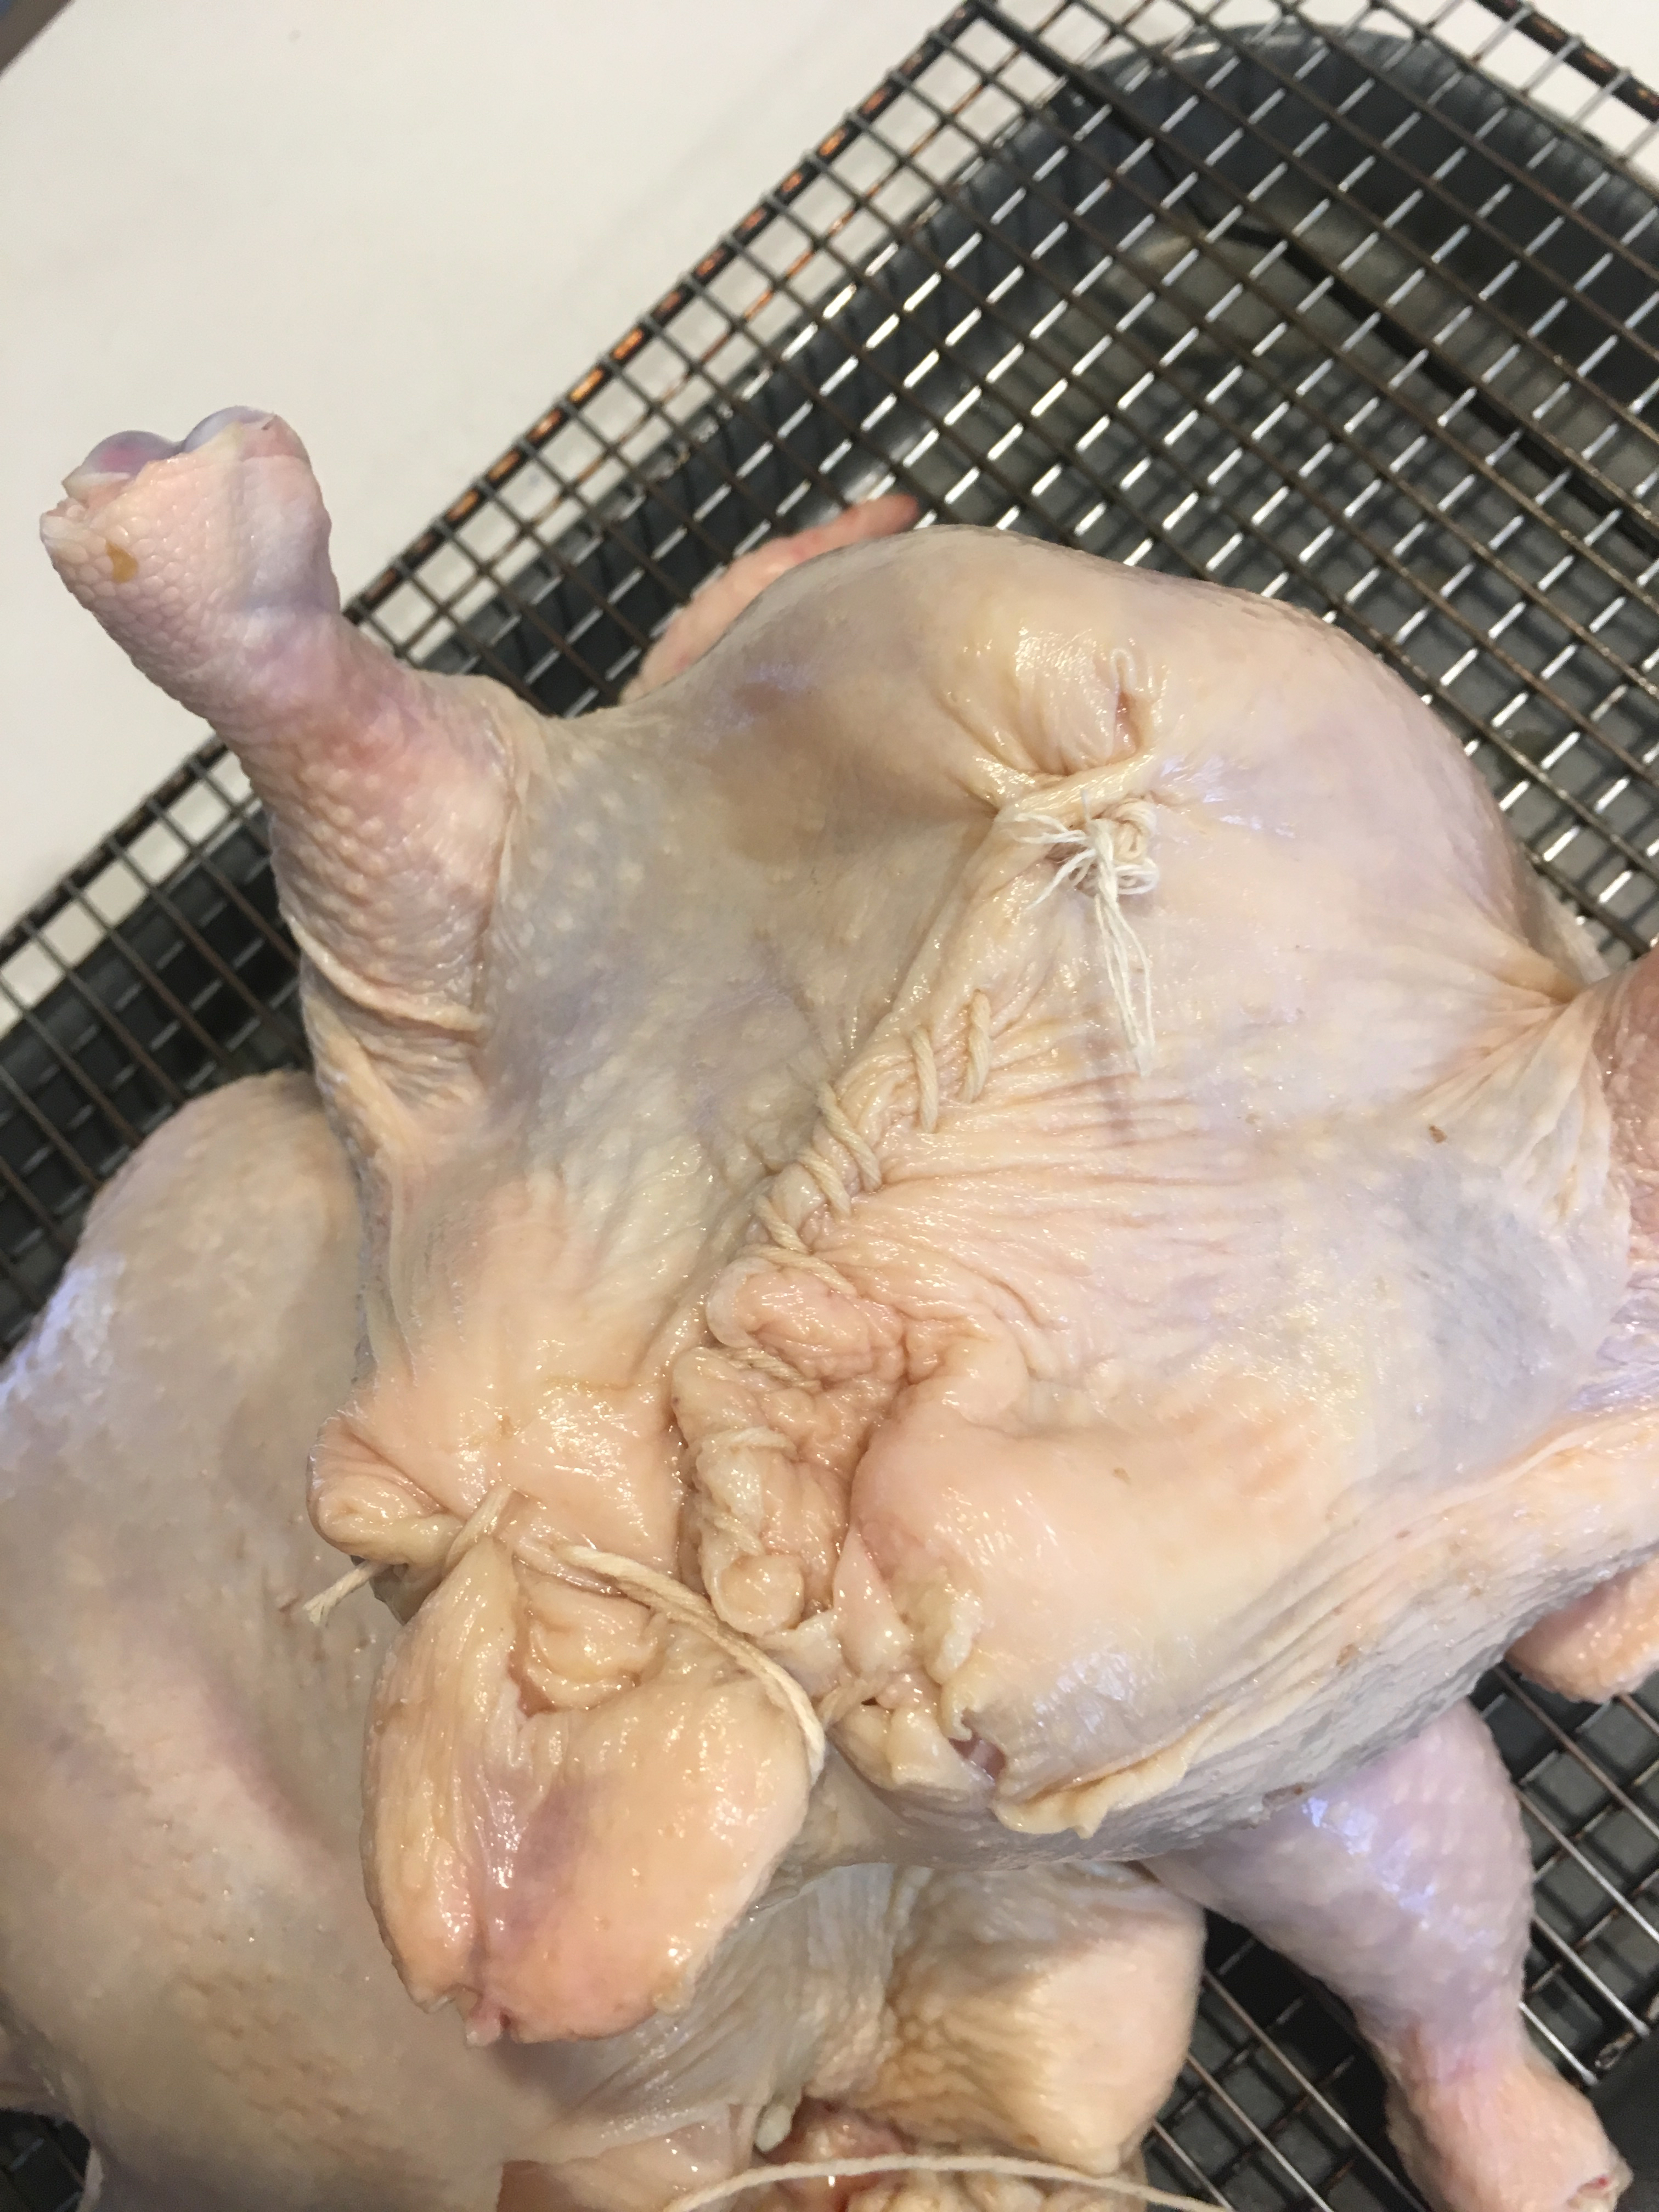
\includegraphics[width=0.25\textwidth]{\imageDir/\fileName/IMG_3217.jpg} &
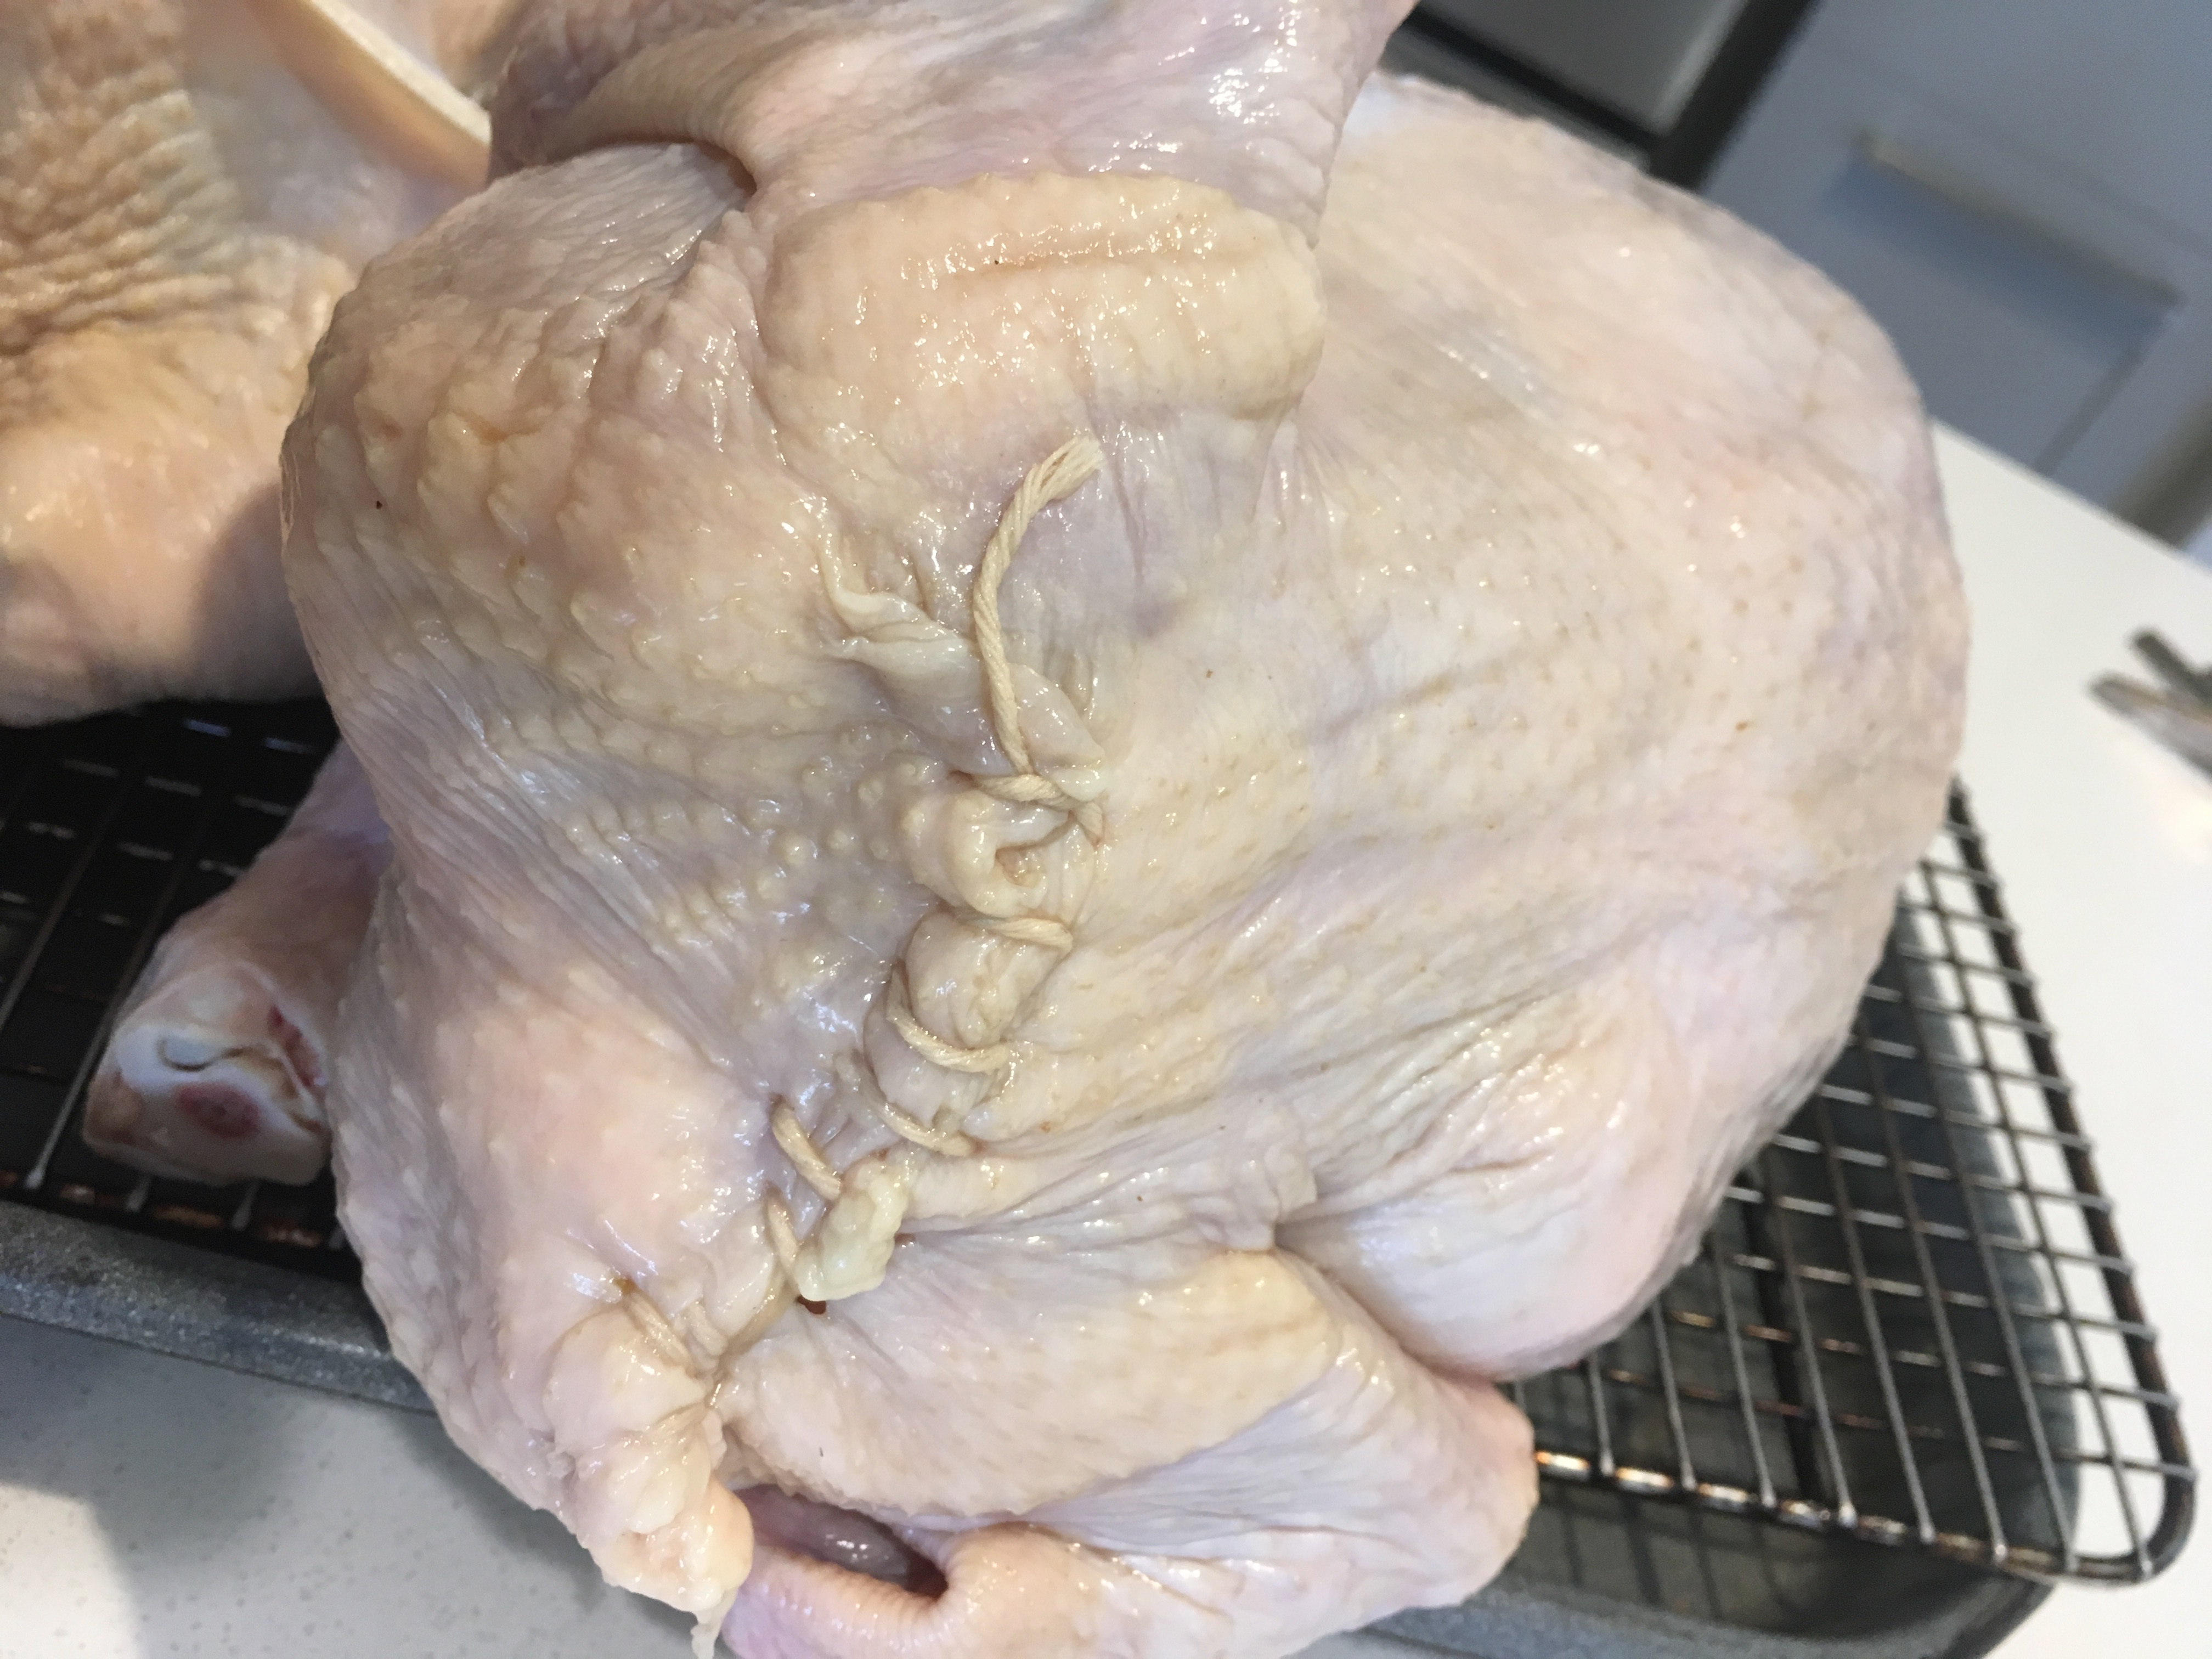
\includegraphics[width=0.25\textwidth]{\imageDir/\fileName/IMG_3218.jpg} &
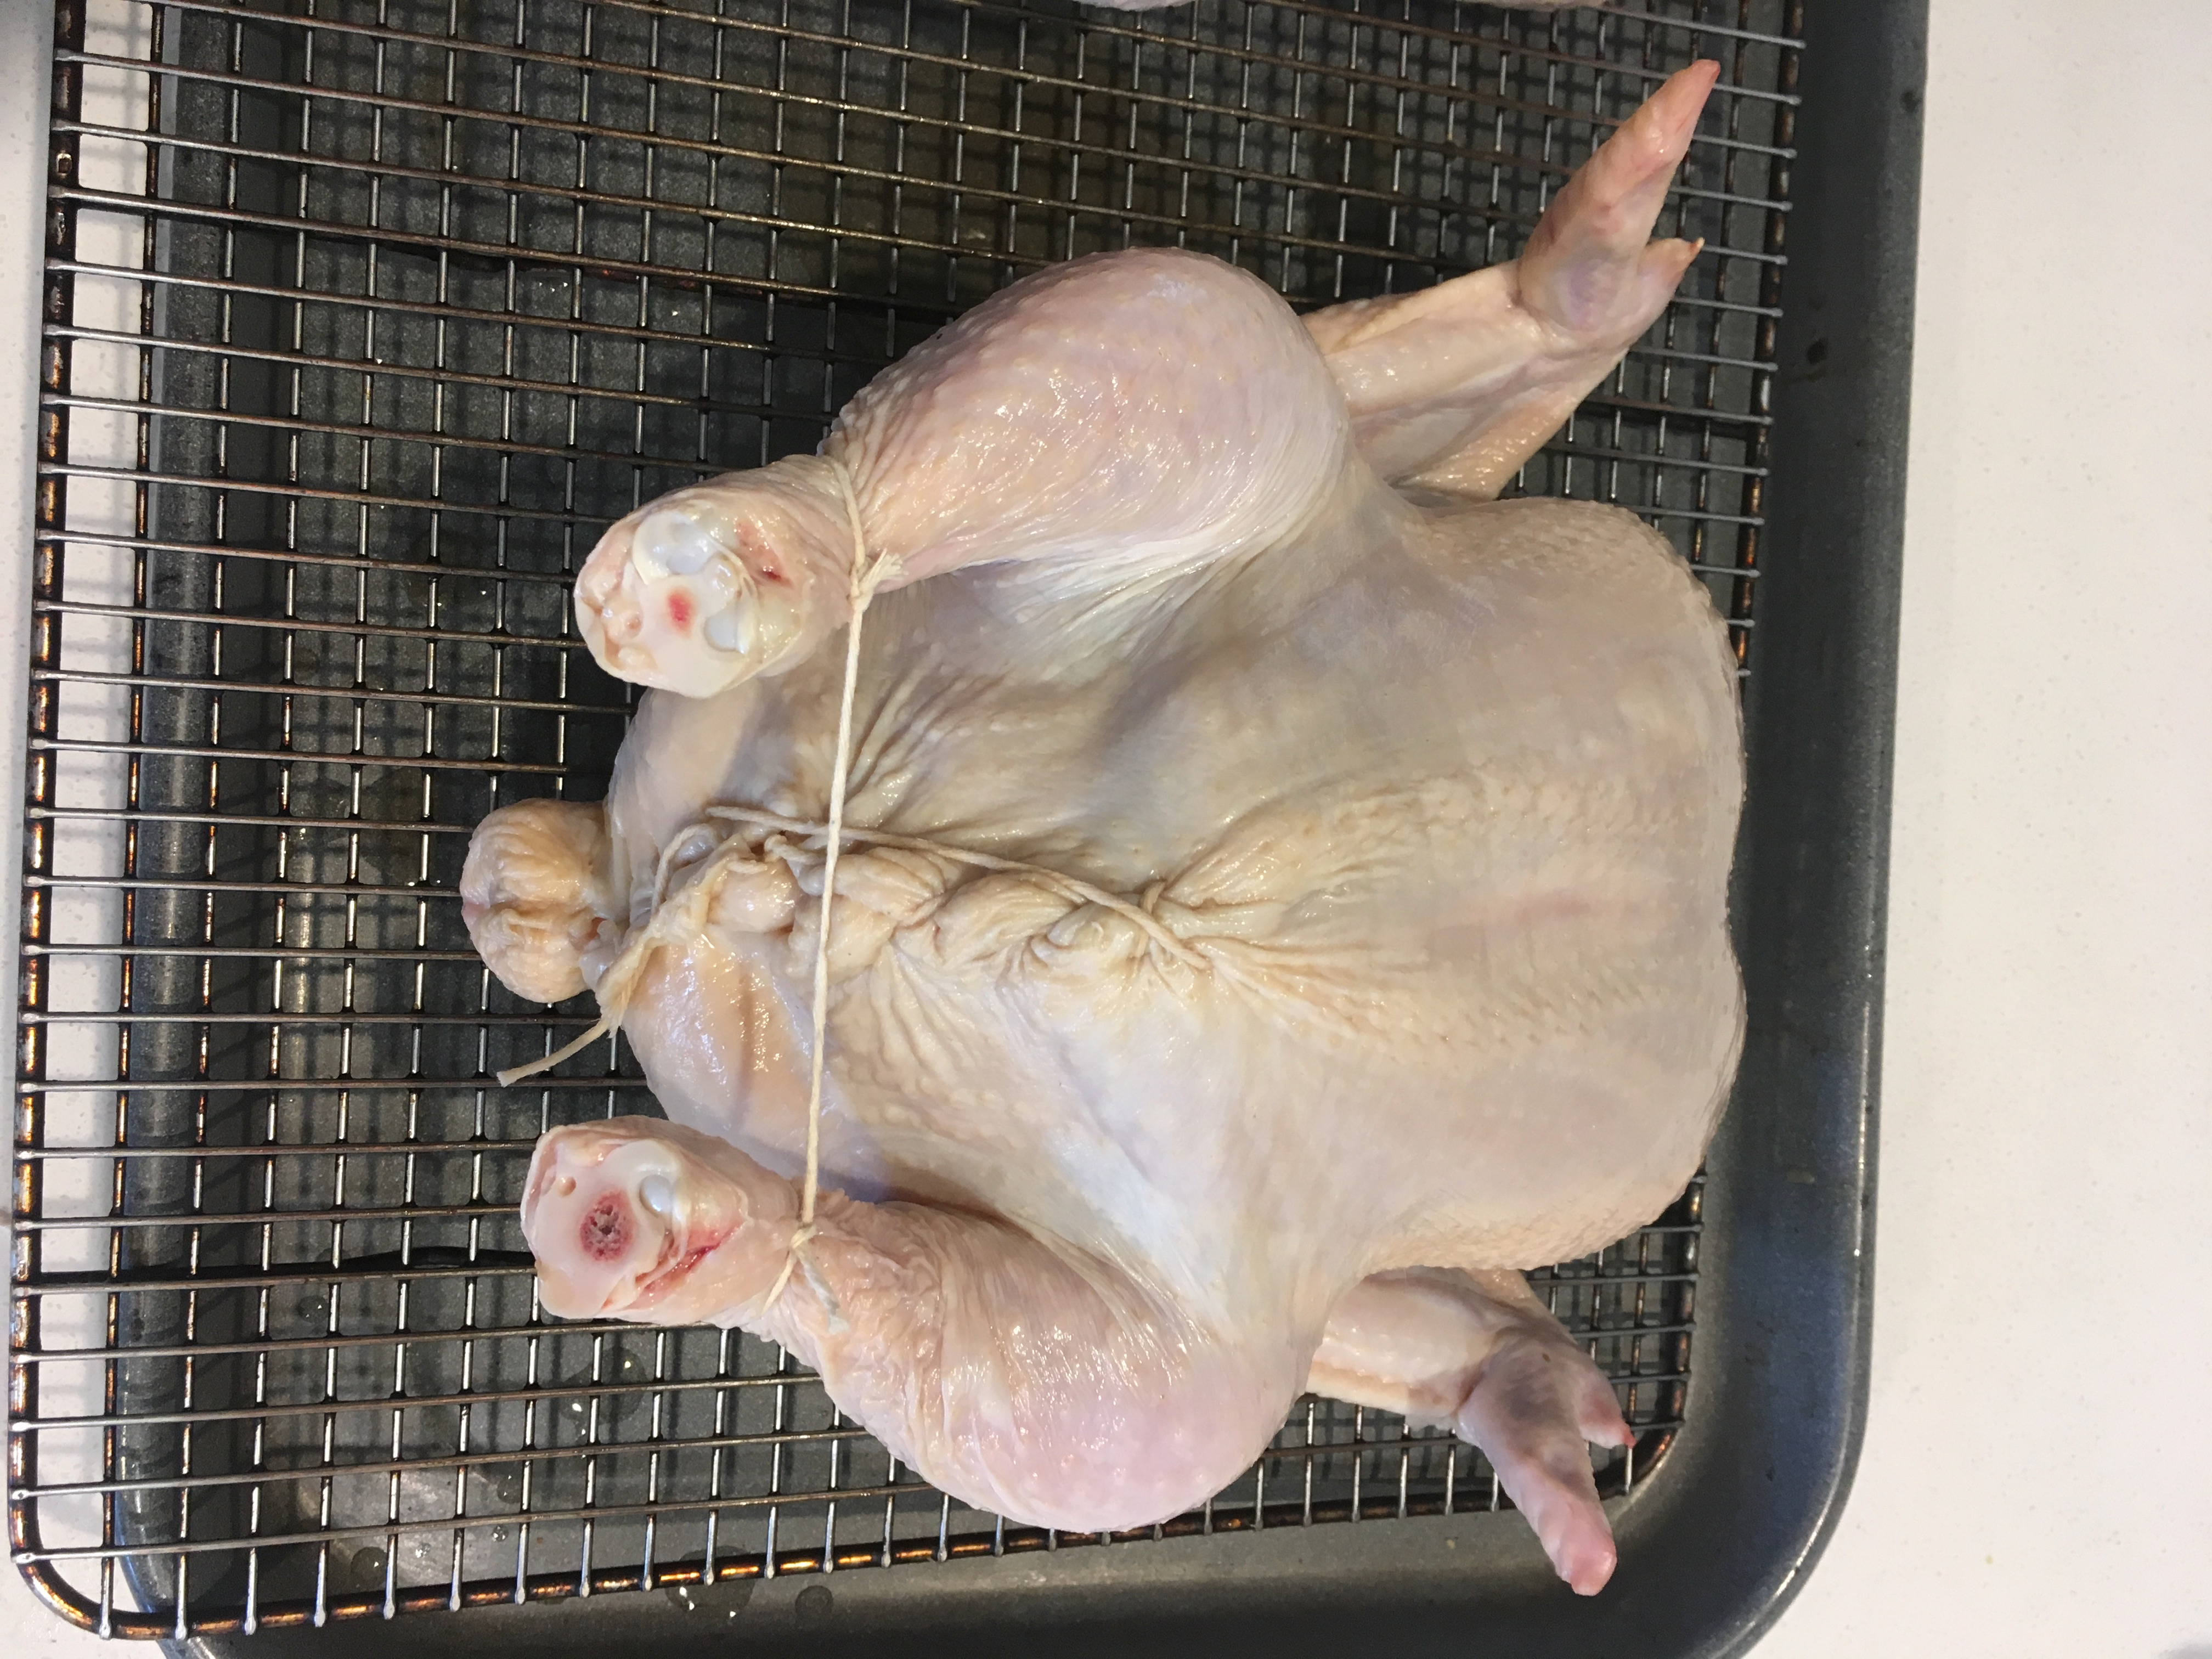
\includegraphics[width=0.25\textwidth]{\imageDir/\fileName/IMG_3219.jpg} \\
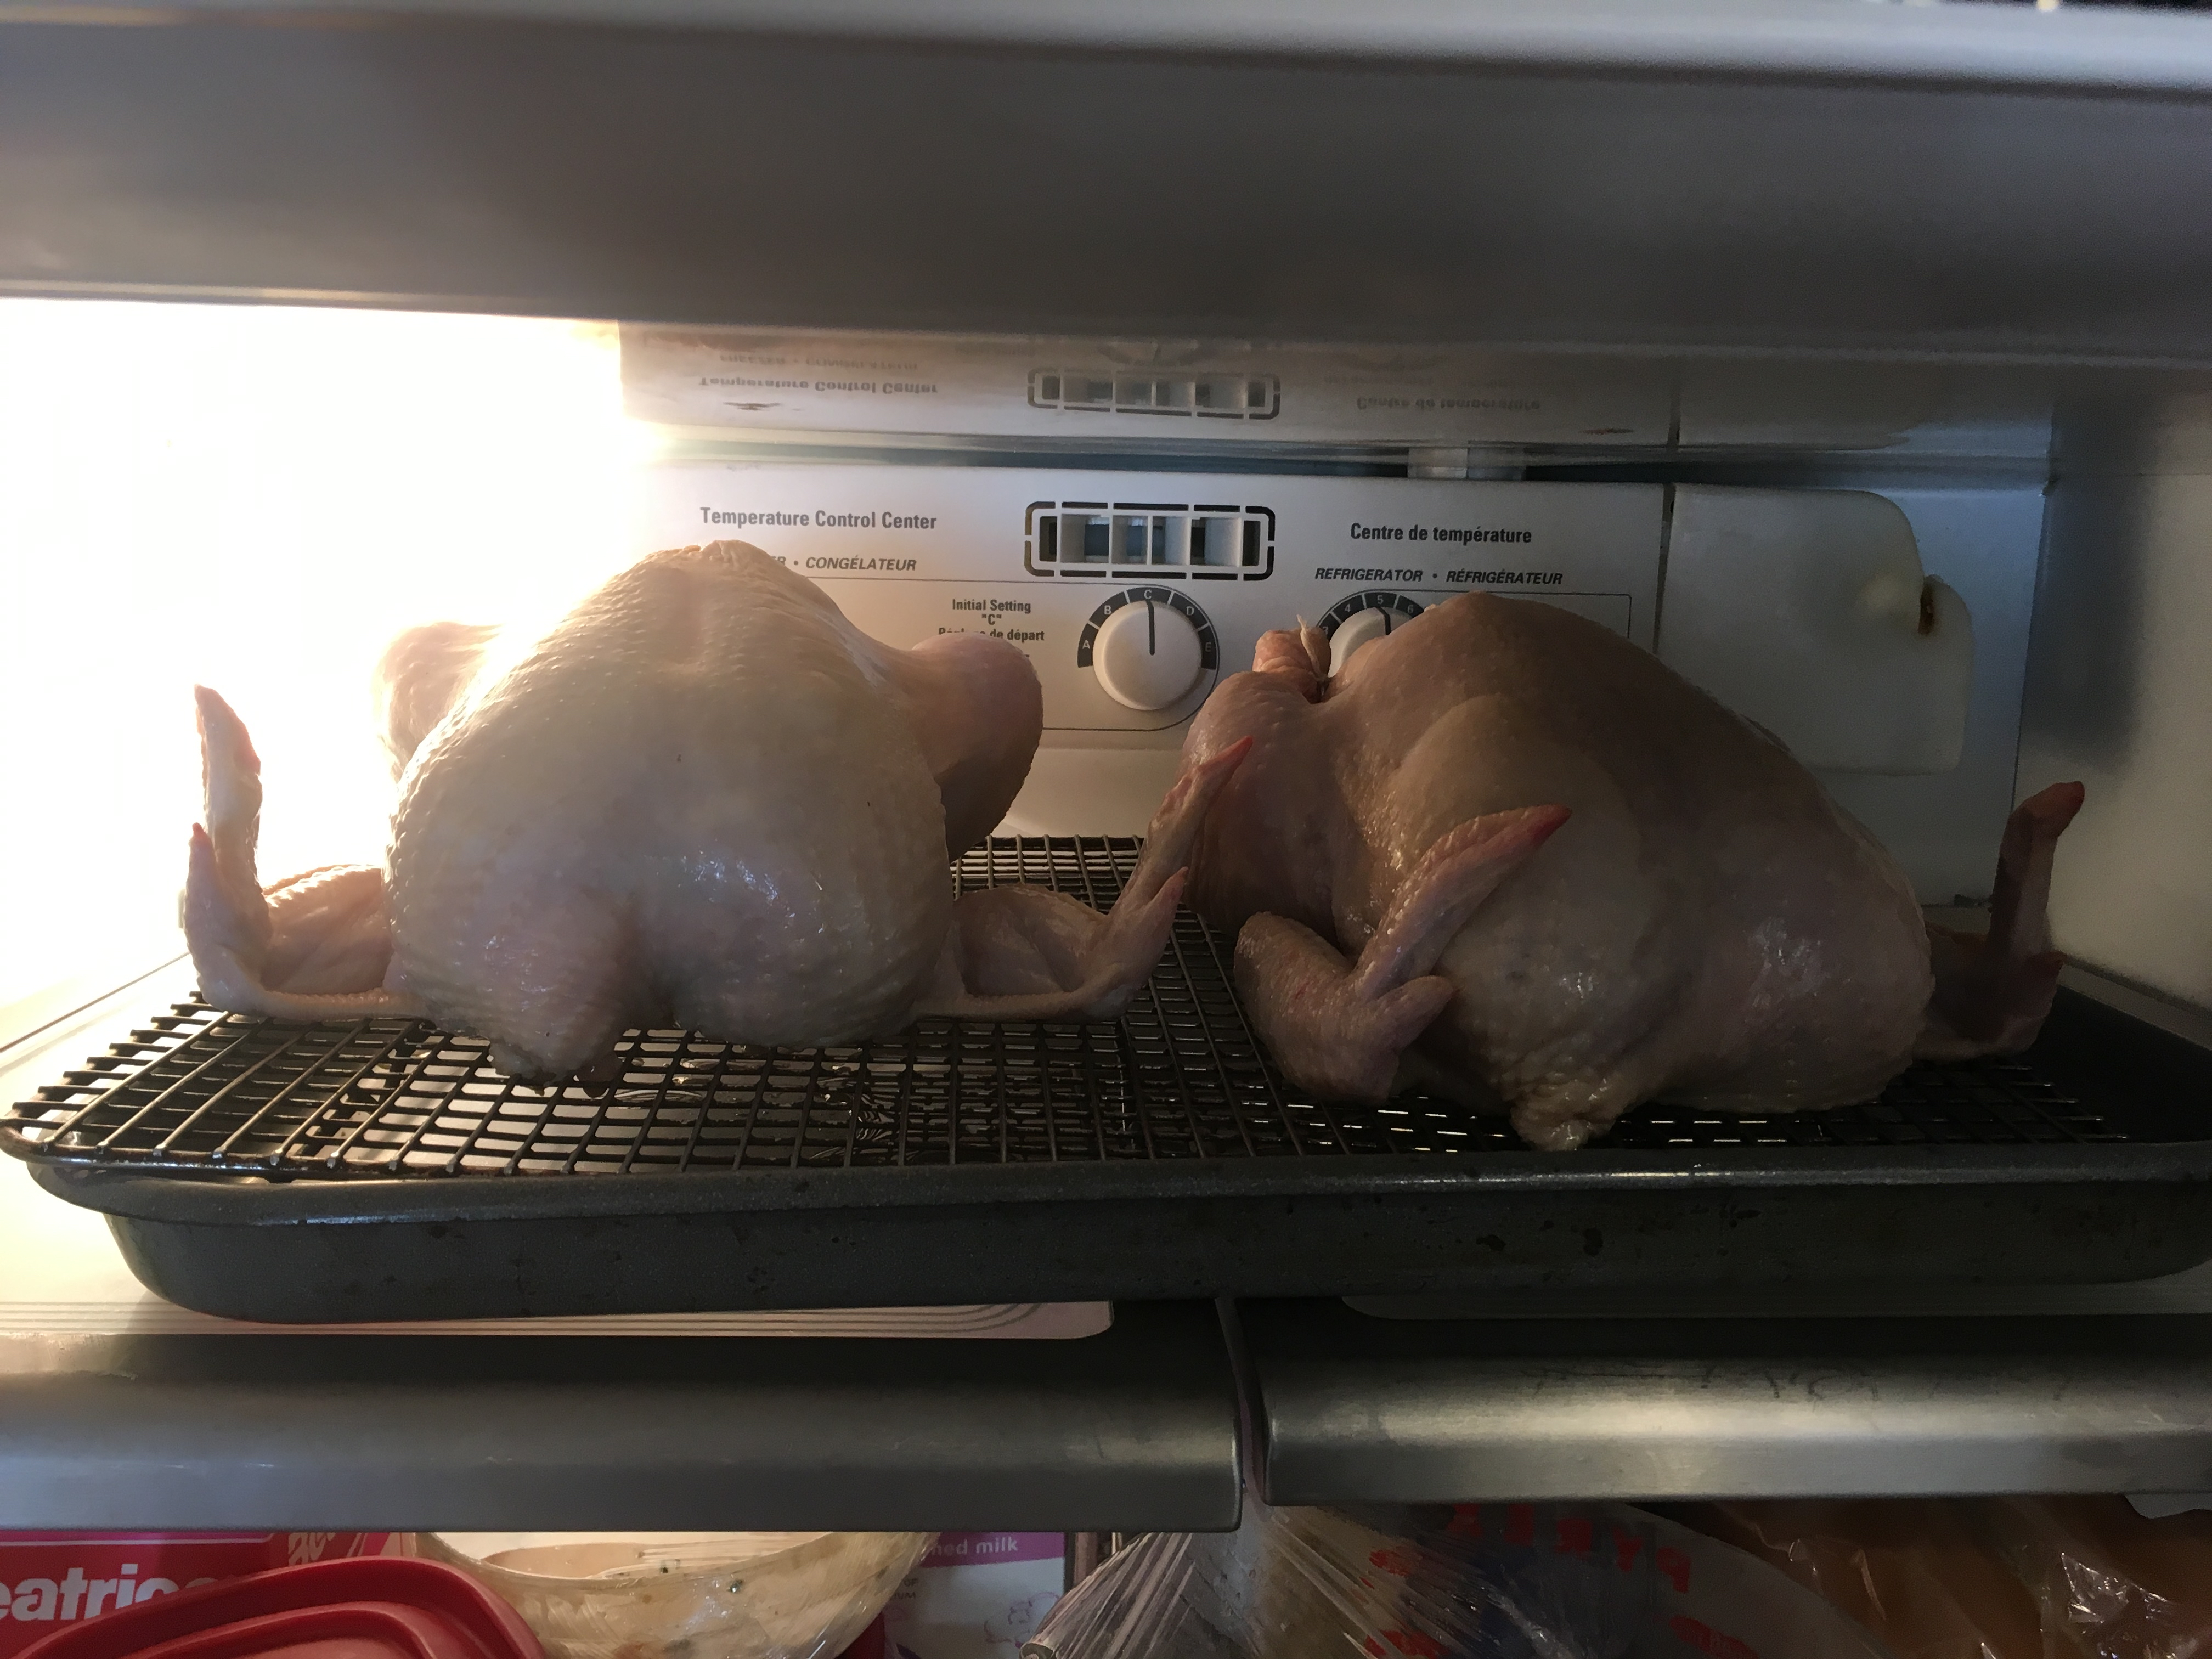
\includegraphics[width=0.25\textwidth]{\imageDir/\fileName/IMG_3220.jpg} &
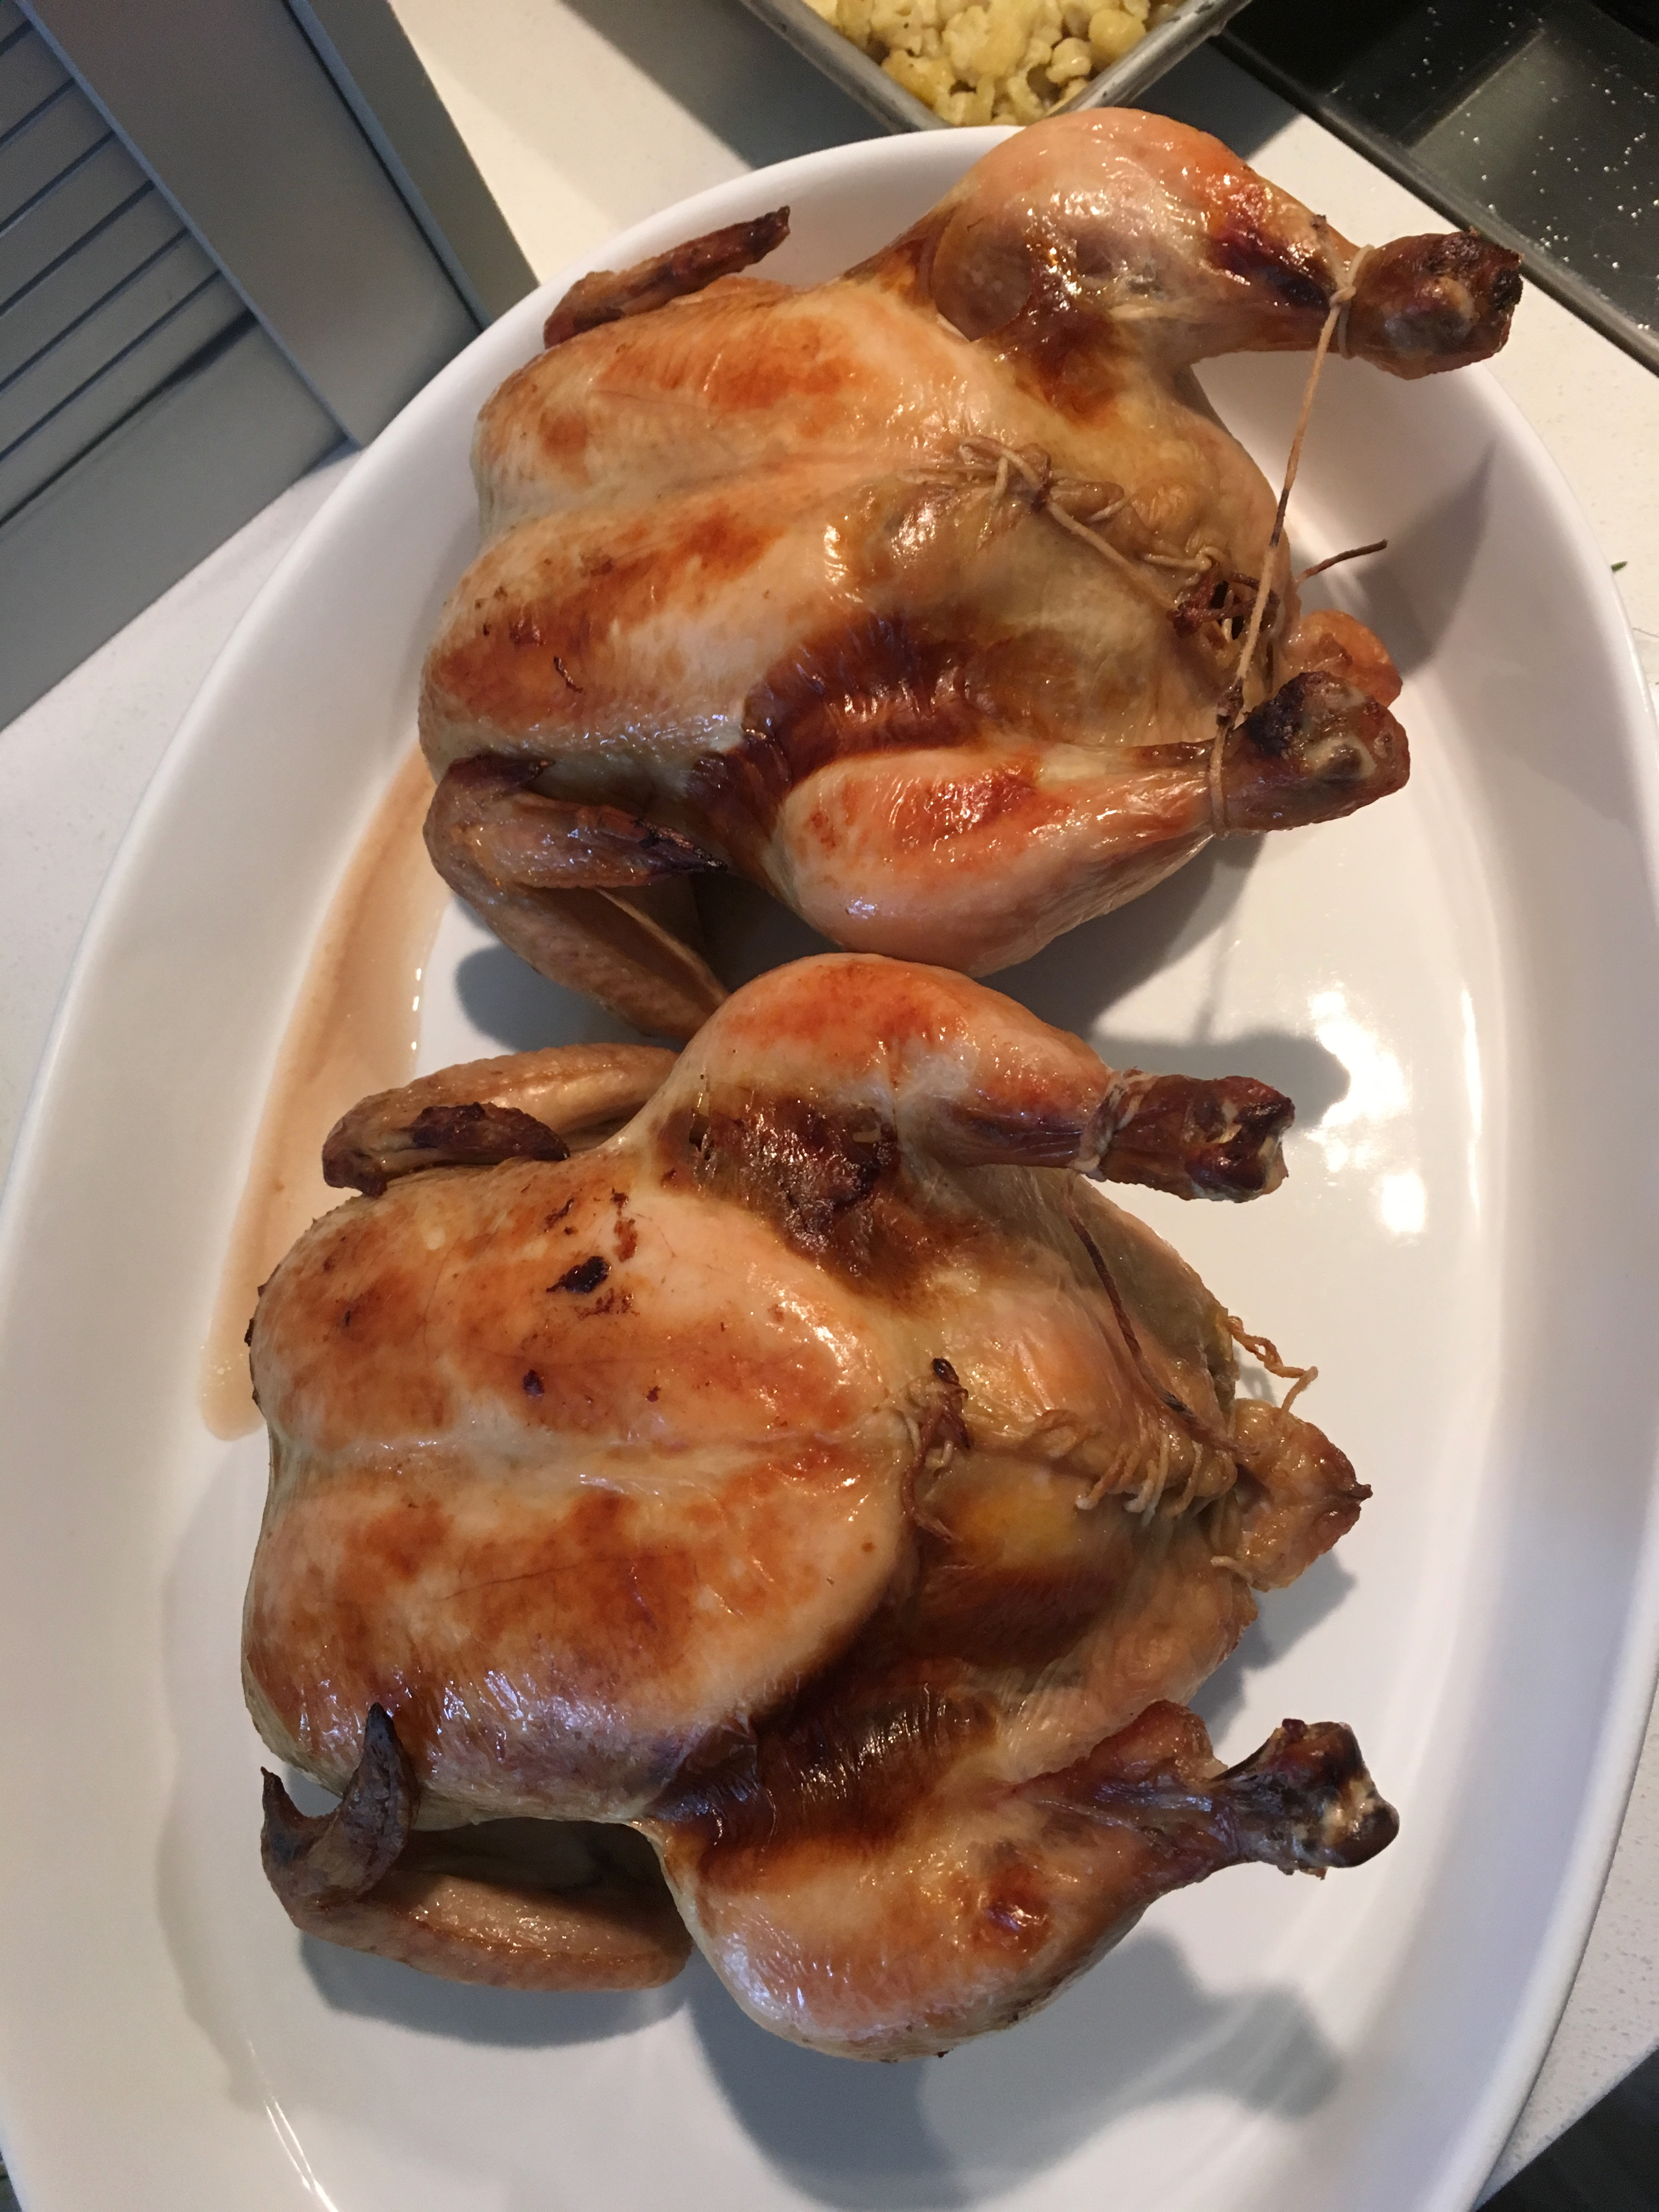
\includegraphics[width=0.25\textwidth]{\imageDir/\fileName/IMG_3228.jpg} \\
\end{tabular}
\end{table}

\end{document}



